\documentclass{book}
\usepackage[utf8]{inputenc}
\usepackage[spanish]{babel}
\usepackage{amsmath,amssymb,amsfonts} %Fonts de AMS
\usepackage{mathbbol} %Font para matrices como la identidad
%%Formato de hoja%%
\usepackage[margin=2cm]{geometry}

%%Imagenes%%
\usepackage{graphicx}
\usepackage{wrapfig}
\usepackage{caption}
\usepackage{subcaption}
\graphicspath{{./fig/}}
\usepackage{float}

%%Ecuaciones y teoremas
\numberwithin{equation}{section} %Número de ecuación por sección

\newtheorem{definition}{Definición}[chapter]
\newtheorem{axiom}{Axioma}[chapter]
\newtheorem{law}{Ley}[chapter]
\newtheorem{principle}{Principio}[chapter]
\newtheorem{postulate}{Postulado}[chapter]
\newtheorem{collorary}{Colorario}[chapter]
%\setcounter{\thelaw}{0}

\title{Notas de Física 4}
\author{S. Schiavinato}
\date{}

\begin{document}
\maketitle
\tableofcontents

\chapter{Termodinámica}
\section{Definiciones básicas}
La termodinámica es la rama de la física encargada de comprender relaciones entre propiedades, que pueden no tener conexión alguna previo al análisis, sin dar una lógica causal.
De esa forma llega a poner límites a los procesos, en vez de explicar el proceso.
\begin{definition}[Sistema]
Toda región del universo dispuesta para el estudio del problema se denomina \emph{sistema}.
Todo el resto se denomina \emph{ambiente} o \emph{entorno}.
El borde del sistema se denomina \emph{contorno}; si este no permite el paso de materia se denomina \emph{abierto}, si no se denomina \emph{cerrado} (aunque esta definición es más amplia a la interacción de energía).
\end{definition}
\begin{definition}[Variables termodinámicas]
Son propiedades o magnitudes físicas necesarias para describir el proceso a estudiar.
Salvo la temperatura, la mayoría de estas magnitudes son de origen externo a la termodinámica.
La variables que dependan del tamaño del sistema se llaman \emph{extensivas}, que notamos en general como $X_i$, y las que no dependen del tamaño del sistema se llaman \emph{intensivas}, notadas como $X_i$.
\end{definition}
\begin{definition}[Estado] Habiendo definidas todas las variables termodinámica de un sistema decimos que el \emph{estado} del sistema está definido. \end{definition}
\begin{definition}[Equilibrio]
Un sistema está en equilibrio si y sólo si para cambiar el estado es necesario un cambio del ambiente, por lo que en el caso estacionario (que no hay flujos constantes de entrada y de salida) las variables se mantienen constantes.
Si el sistema está estacionario además no tiene información de cómo llegó el sistema a ese estado de equilibrio.
\end{definition}
La termodinámica podemos plantearla de varias formas posibles, nosotros vamos a mezclar algunas leyes con los postulados, pero solamente con los postulados es suficiente para formalizar toda la teoría física.
El primer postulado es necesario para darle sustento físico a la teoría, ya que a priori pueden no existir los estados de equilibrio
\begin{principle}[Existencia de los estados de equilibrio]
Existen los estados de equilibrio para sistemas caracterizados por finitas variables termodinámicas extensivas.
\end{principle}
La elección de variables termodinámicas de un sistema está sólamente condicionada por la experiencia física, por lo que es relevante para el sistema según el observador.
\begin{law}[Cero: Transitividad del equilibrio]
Si hay dos sistemas $A$ y $B$ en equilibrio térmico, es decir misma temperatura, y otro sistema $C$ está en equilibrio con $B$, entonces $A$ y $B$ están en equilibrio
\end{law}
\section{Primera Ley}
Joule en XXXX dispuso en una caja adiabática un líquido (uso agua, mercurio y otros materiales) con un método mecánico para revolverlo, como vemos en la figura \ref{fig:primera_ley}.
\begin{wrapfigure}{r}{0.35\linewidth}
\centering
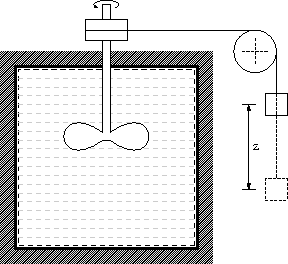
\includegraphics[width=0.35\textwidth]{primera_ley}
\caption{Experiencias de Joule}
\label{fig:primera_ley}
\end{wrapfigure}
La idea de la experiencia que el cuerpo cae a velocidad constante, por lo que toda la energía potencial se transfiere efectivamente al medio fluido (y como tiene una límite adiabático es la \emph{única} forma de alterar el sistema), y observar el cambio de temperatura del medio.
Joule observó que dicho cambio de temperatura sólo depende de la altura del cuerpo, es decir, de la energía potencial del cuerpo.
Además observó el mismo cambio de estado cambiando el mecanismo de ingreso de energía, por ejemplo por fricción o por una corriente eléctrica, o el sistema en si, un fluido diferente como el mercurio.
Es decir, Joule encontró que existe una magnitud conservativa (que sólo depende del estado inicial y final) independiente de la naturaleza del sistema que está asociada a la energía externa ingresante a dicho sistema, que llamamos \emph{energía interna} $U$
\begin{definition}[Energía interna]
La energía interna corresponde al trabajo adiabático efectuado en el sistema
\begin{equation}
dU = - d'W_{ad}
\end{equation}
La energía del sistema sólo depende del estado inicial y final, es decir
\begin{equation}
\oint dU = 0
\end{equation}
\end{definition}
Como ya mencionamos arriba, la energía $U$ es conservativa, así que debe existir una ley de conservación asociada.
Continuando con sus experiencias, Joule observó que la energía mecánica necesaria para llevar de un estado a otro sólo con transferencia de calor son equivalentes.
Es decir, Joule disponía de un cuerpo $B$ y otro $A$, con diferentes temperaturas, y al unirlos con una interface diatérmica hubo un cambio de estado; este cambio de estado corresponde a un valor de calor que es equivalente al trabajo necesario para llevar la temperatura del sistema que se enfrió a su temperatura al principio de la experiencia.
Con esta deducción Joule estableció la naturaleza del calor: es un tipo de energía
\begin{law}[Primera: Conservación de la energía]
El primer principio o postulado de la termodinámica determina que el trabajo efectuado en el sistema en condiciones adiabáticas sólo depende de las condiciones iniciales y finales, o dicho de otra manera, el trabajo entre dos estados de equilibrio es independiente del proceso efectuado (siempre en condiciones adiabáticas). En caso de tener una transformación no adiabática, la diferencia entre el trabajo efectuado y la energía interna es el calor
\begin{equation}
\Delta U = Q - W \Rightarrow dU = \delta Q - \delta W
\end{equation}
\end{law}
La diferencia entre $d$ y $\delta$ es que el trabajo y el calor si depende de la transformación, pero la energía interna no. En matemática los $d$ se llaman exactos, y verifican que sus magnitudes son conservativas.
\subsection{Trabajos generalizados}
La conservación de la energía no sólo funciona a sistemas simples, si no se ha encontrado sistema donde no se aplique. Pero para eso necesitamos generalizar el concepto de trabajo, usando el concepto de magnitud extensiva e intensiva
\begin{definition}[Variable extensiva e intesiva]
Una variable termodinámica extensiva $X$ corresponde a una magnitud que varia con el cambio del sistema, en general aumenta si aumenta el sistema, mientras una variable intensiva $Y$ no depende del tamaño del sistema.
\end{definition}
Ahora vamos a pasar a definir el trabajo generalizado, a partir del concepto de trabajo mecánico, que corresponde a $dW = F dx$, es decir el producto de una fuerza, que en el formalismo termodinámico corresponde a una variable intensiva, por un desplazamiento, una variable extensiva. De esta forma
\begin{definition}[Trabajo generalizado]
El trabajo \textit{de configuración} corresponde al trabajo necesario para llevar de un estado de equilibrio a otro estado de equilibrio de forma reversible, que se debe expresar como
\begin{equation}
d'W = \sum_i Y_i dX_i
\end{equation}
con $Y_i$ una variable intensiva y $X_i$ una variable extensiva
mientras que el trabajo \textit{disipativo} corresponde al efectuado de forma irreversible y no puede ser expresado con combinación lineal de diferenciales.
\end{definition}
Veremos que en concepto de trabajo de configuración podemos incluir el calor, cuando definamos la entropía.
Las variables que determinan un trabajo generalizado de configuración se denominan \emph{variables conjugadas}.
\section{Segunda ley}
En este principio, desarrollado antes que el primer principio históricamente, determina una imposibilidad de la naturaleza, además trae consigo una asimetrí temporal a los estados; determina la flecha del tiempo.
Pero ya vamos a ver todo eso.
Primero observemos el enunciado de Kelvin, que finalmente escribiremos como un postulado
\begin{law}[Enunciado de Kelvin]
No es posible tener una máquina térmica ciclica que tenga como único resultado eliminar calor de una fuente y transformarlo en trabajo.
\end{law}
De este principio nos queda definir que es una máquina térmica ciclica
\begin{definition}[Maquina térmica ciclica]
Proceso que altera el sistema desde un estado hasta otros estados, finalmente retornando al mismo estado inicial
\begin{figure}[H]
\centering
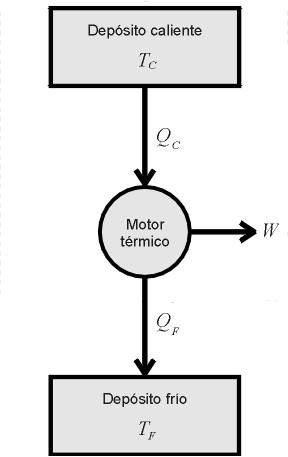
\includegraphics[width=0.18\textwidth]{motor}
\caption{Esquema simbólico del motor térmico}
\end{figure}
\end{definition}
El enunciado de Kelvin nos indica que la eficiencia de los motores no puede ser del 100\%, ya que
\begin{equation}
\eta = \frac{W}{Q_{in}} < 1
\end{equation}
\begin{collorary}[Existencia de la entropía]
Para todo sistema existe una función $S = S(U, \{X_i\})$, es decir función de las variables extensivas del sistema (en general $U$, $V$ y $N$), tal que una transformación isoentrópica reversible ($dS = 0$) implique que la transformación es además adiabática, es decir $dS = 0 \Leftrightarrow \delta Q = 0$.
Además de la definición se deduce que es una función de estado, ya que dado un estado tiene un valor definido independiente del camino ejecutado (a menos de una constante para todos los estados).
\end{collorary}
Para demostrar la existencia de la entropía, construimos un espacio dado por las variables extensivas $\{U,X_i\}$ (que vamos a tomar, para simplificar las ideas, $\{U,V,N\}$).
En ese espacio definimos un punto $A$, y otro $A'$ separados por una curva de $\{X_i\}$ constante.
Esos dos puntos están unidos por una curva no adiabática, es decir al tener diferente energía $U(A) \neq U(A')$, pero a $\{X_i\}$ constante, es necesario que ese cambio energético sea en forma de calor, es decir
\[U(A') = U(A) + Q_{A \to A'}.\]
Ahora si volvemos de $A'$ a $A$ por un camino adiabático, por lo que
\[U(A) = U(A') - W_{A' \to A},\]
pero efectuamos un ciclo cerrado donde transformamos calor en trabajo (ya que asumimos que pasar de $A$ a $A'$ implica agregar trabajo, es decir la curva es con $U$ creciente), siendo un proceso imposible según el enunciado de Kelvin.
Esto define conjuntos de puntos accesibles con procesos adiabáticos, que forman superficies que no se interfieren (por lo que ya vimos recién).
Un esquema de lo que efectuamos acá se presenta en la figura \ref{fig:segunda_ley_espacio}, pero considerando otros puntos del espacio.

\begin{figure}[H]
    \centering
    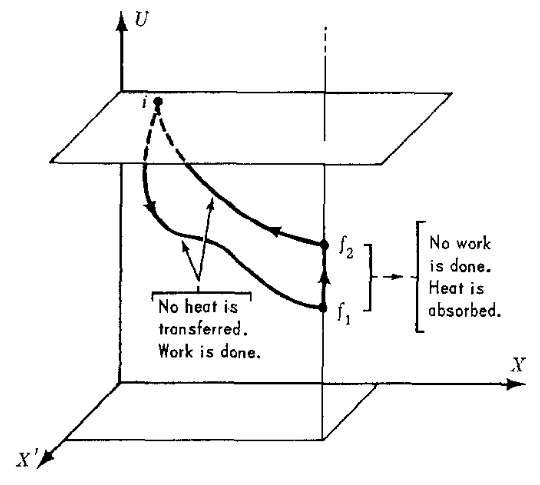
\includegraphics[width=0.6\textwidth]{segunda_ley_espacio}
    \caption{Diagrama del argumento para seleccionar puntos inalcanzables por transformaciones adiabáticas}
    \label{fig:segunda_ley_espacio}
\end{figure}

Esas superficies las vamos a parametrizar con \[S(U,\{X_i\}) = c,\] siendo S una función continua suave (ya que asumimos que las superficies son suaves), la \emph{entropía}.
Por definición, las superficies de nivel de $S(U,\{X_i\})$ son adiabáticas, y además podemos escribir a la energía como
\[dU = \frac{\partial U}{\partial S} dS + \frac{\partial U}{\partial X_i} dX_i = \delta Q - \delta W\]
de lo que se deduce automáticamente que el calor debe ser (ya que si $dS = 0$ entonces es necesario que $\delta Q = 0$)
\begin{equation}
\delta Q = \frac{\partial S}{\partial U} dS
\end{equation}
Si elegimos $\lambda = \frac{1}{T}$ a priori, podemos ver después que realmente es una temperatura, verificando la ley cero y la noción que tenemos de ella. Esto determina que
\begin{equation}
\frac{1}{T} = \left.\frac{\partial S}{\partial U}\right|_{X_i}
\end{equation}
\begin{collorary}[Desigualdad de Clausius]
Para una transformación cualquiera se verifica que \[T dS \geq \delta Q\] siendo una igualdad si el proceso es reversible
\end{collorary}
Para demostrar este colorario utilizamos nuevamente dos estados $A$ y $A'$ en el espacio $\{U,X_i\}$ unidos por una transformación (puede ser reversible o no).
En esta transformación hay un intercambio de calor $\delta Q$, y luego se genera una transformación adiabática a un estado nuevo $B$, conectado con $A$ por medio de una curva $\{X_i\}$ constante.
El calor en todo este ciclo es
\[\delta Q + \delta Q_{A' \to B} + \delta Q_{B \to A} = \delta Q + 0 - T dS.\]
Ese último despeje deriva que el proceso de $B$ a $A$ es reversible, por lo que $U(B) - U(A) = dU = T dS$, al ser las demás variables constantes. De Kelvin podemos deducir que el calor total debe ser negativo, ya que al haber calor positivo en el primer proceso y calor negativo en el segudo debió haber un trabajo positivo en el intermedio, por lo que finalmente se llega a que
\[\delta Q \leq T dS\]
para cualquier transformación.
Además podemos ver que $\lambda = \frac{1}{T}$, es factor integrante, es realmente una temperatura.
Para eso tomamos dos sistemas $1$ y $2$ en contacto térmico.
El sistema $1$ está a mayor temperatura que el sistema $2$. La entropía ya sabemos que es extensiva y aditiva (como la energía), por lo que
\[dS_{T} = dS_1 + dS_2 = -\frac{Q}{T_1} + \frac{Q}{T_2} = Q \left(\frac{1}{T_2} - \frac{1}{T_1}\right).\]
De la desigualdad de Clausius obtenemos que $T dS \geq 0$ por lo que para que la temperatura fluya de $1$ a $2$ se debe dar que $T_1 > T_2$.
Lo mismo podemos hacer para $T_2 > T_1$. Queda demostrado que el factor integrante es una temperatura, y además es imposible que se de el flujo de calor de otra forma, es decir
\begin{collorary}[Enunciado de Clausius]
No es posible mover con una máquina térmica cíclica calor de una fuente fría a una caliente, sin agregar trabajo.
\end{collorary}
con lo que cerramos los enunciados históricos de la segunda ley.
Nos queda deducir el teorema de Carnot para una máquina ciclica, que es fácil de deducir ya que sabemos que
\[\eta = \frac{W}{Q_{\in}} = \frac{Q_{in} - Q_{out}}{Q_{in}} = 1 - \frac{Q_{out}}{Q_{in}} \leq 1 - \frac{T_{f} \Delta S}{T_C \Delta S}\]
lo que finalmente se deduce en
\begin{collorary}[Teorema de Carnot]
El trabajo de cualquier máquina térmica, reversible o no, es menor igual a la unidad menos la relación entre la temperatura del reservorio frio y la del reservorio caliente\
\begin{equation}
\eta \leq 1 - \frac{T_F}{T_C}
\end{equation}
\end{collorary}
\section{Propiedades intensivas, relaciones}
Hemos asumido en los apartados anteriores que la energía y la entropía son funciones extensivas, por lo que son homogeneas de primer orden
\[ U(\lambda S, \{\lambda X_i \}) = \lambda U(S,\{X_i\}) \]
Si derivamos respecto a $\lambda$ de ambos términos
\[ \frac{\partial U(\lambda S, \{\lambda X_i\})}{\partial (\lambda S)} \frac{\partial (\lambda S)}{\partial \lambda} + \frac{\partial U(\lambda S, \{\lambda X_i\})}{\partial (\lambda X_i)} \frac{\partial (\lambda X_i)}{\partial \lambda} = U(S,\{X_i\})\]
Si evaluamos en $\lambda = 1$ como caso particular (por el cual no se pierde generalización), obtenemos la siguiente relación
\begin{equation}
U = T S + X_i Y_i
\label{eq:euler}
\end{equation}
donde sabemos que las variables intensivas conjugadas
\begin{equation}
Y_i = \left.\frac{\partial U}{\partial X_i}\right|_{T,X_j}
\end{equation}
La ecuación resultante se denomina ecuación de Euler.
Para la entropía podemos hacer el mismo proceso, obteniendo
\begin{equation}
S = \frac{U}{T} - \frac{Y_i}{T} X_i
\label{eq:euler_entropia}
\end{equation}
Si diferenciamos ambos términos de la ecuación de Euler, y simplificamos obtenemos la siguiente relación
\begin{equation}
S dT - X_i dY_i = 0
\label{eq:gibbs_durheim}
\end{equation}
llamada de Gibbs-Durheim, que nos permite relacionar las variables intensivas entre si.
La ecuación de Gibbs-Durheim impide la existencia de potenciales termodinámicos con variables intensivas solamente.
\section{Potenciales termodinámicos}
Ahora vamos a pasar a encontrar \emph{potenciales termodinámicos}, es decir funciones que en diferentes casos al ser minimizadas o maximizadas nos dan el estado de equilibrio.
Con esta definición ya es claro que la entropía $S = S(U,\{X_i\})$ es un potencial, pero respecto a variables no muy útiles experimentalmente.
También podemos encontrar lo mismo para la energía $U = U(S,\{X_i\})$, que debe ser un mínimo a respecto la entropía y las demás variables extensivas.
Nuevamente vemos que la energía interna así planteada no tiene utilidad experimental, ya que es muy complicado de medir la entropía (en general se la deduce).
Para eso usamos transformadas de Legendre
\subsection{Transformada de Legrendre}
Supongamos que tenemos una función de dos variables (se puede extender a cualquier cantidad de variables) $f(x,y)$ y una variable $z = \left.\dfrac{\partial f}{\partial x}\right|_y$.
Si quiero una función $\tilde{f}(z,y)$, la transformada de Legrende la define así
\begin{equation}
\tilde{f}(z,y) = f(x,y) - \left.\frac{\partial f}{\partial x}\right|_y x = f(x,y) - z\, x
\label{eq:legendre}
\end{equation}
Nos queda demostrar que las derivadas de la función nueva son lo que queremos que sea
\[\frac{\partial \tilde{f}}{\partial z} = \frac{\partial}{\partial z} \left( f(x(y,z),y) - x(y,z) \, z \right) = \frac{\partial f}{\partial x} \frac{\partial x(y,z)}{\partial z} - \frac{\partial x}{\partial z} z - x = z \frac{\partial x}{\partial y} - \frac{\partial x}{\partial y} z - x = - x.\]
La otra derivada la calculamos de la misma forma
\[\left.\frac{\partial \tilde{f}}{\partial y}\right|_z = \frac{\partial f}{\partial y} + \frac{\partial f}{\partial x} \frac{\partial x}{\partial y} - \frac{\partial x}{\partial y} z = \frac{\partial f}{\partial y}.\]
Estas dos relaciones las podemos unir en
\begin{equation}
\begin{gathered}
\left.\frac{\partial \tilde{f}(z,y)}{\partial z}\right|_y = - x\\
\left.\frac{\partial \tilde{f}(z,y)}{\partial y}\right|_z = \left.\frac{\partial f(x,y)}{\partial y}\right|_x
\end{gathered}
\end{equation}
El diferencial de la función $\tilde{f}$ es por lo tanto
\begin{equation}
d\tilde{f} = -x dz + \frac{\partial f}{\partial y} dy
\end{equation}
\subsection{Energias libres y entalpia}
Con la definición de transformación de Legandre, pasemos a encontrar algunas funciones derivadas de la energía $U = U(S,\{X_i\}$.
Para empezar encontremos una función $F = F(T,\{X_i\})$, es decir intercambiando entropía con temperatura, siendo una función más fácil de encontrar experimentalmente.
Sabemos que $T = \dfrac{\partial U}{\partial S}$, por lo que
\[ F(T,V,\{X_i\}) = U[T,V,\{X_i\}) U - S \frac{\partial U}{\partial S}\]
\begin{equation}
\begin{gathered}
F = U - T\,S \\
dF = - S\,dT - p d V - Y_i dX_i
\end{gathered}
\label{eq:energia_helmoltz}
\end{equation}
función que llamamos energía libre de Helmholtz.
Si trabajamos sobre el diferencial de la energía libre, usando la desigualdad de Clausius, tenemos que
\[dF = dU - T dS - SdT = (\delta Q - T dS) - \delta W - S dT \leq - \delta W - S dT\]
que para el caso de temperatura constante $dT = 0$ nos queda
\begin{equation}
dF \leq - \delta W
\end{equation}
es decir que el trabajo maximo extraíble a temperatura constante depende solamente de la energía libre, como bien su nombre describe.
El máximo se dará en el caso extraíble, donde $dF = - \delta W$
Además sin el trabajo es nulo, el estado de equilibrio se dará cuando
\begin{equation}
dF \leq 0
\end{equation}
es decir cuando sea un mínimo de la energía libre.
Por esto es que se denominan potenciales termodinámicos
Lo mismo podemos hacer con la presión y la tempratura, es decir
\begin{equation}
\begin{gathered}
G = U[T,p,\{X_i\}] = U - T\,S + p \, V \\
dG = S\,dT + V dp - X_i dY_i
\end{gathered}
\label{eq:energia_gibbs}
\end{equation}
Esta función se llama energía libre de Gibbs, o función de Gibss.
Esta función es en particular útil para transformaciones de fase, ya que ocurren a temperatura y presión constante, al menos en las fases "comunes".
Además si el trabajo generalizado es solamente
\[\delta W = p dV - \mu dN\]
entonces la energía libre de Gibbs a temperatura y presión constante es
\begin{equation}
G = \mu N
\end{equation}
Veamos el diferencial de esta función
\[dG = dU - T dS - S dT + p dV + V dp + X_i dY_i = (\delta Q - T dS) - (\delta W - p dV) - S dT + V dp + X_i dY_i \leq V dp - S dT - (\delta W - p dV\]
Si la temperatura y la presión son constantes entonces
\[dG \leq \delta W - p dV = p_{ext} dV - p dV = 0\]
donde asumimos que la transformación es cuasiestacionaria, por lo que finalmente deducimos que la energía libre de Gibbs es un mínimo, siendo un potencial termodinámico.
De forma general, cualquier función que sea una transformación de Legendre de la energía será minimo, en caso de que las variables acordes estén fijadas. Esto nos permite generar toda una familia de funciones, pero las más comunes ya las presentamos
Nos queda la entalpía, que corresponde a
\begin{equation}
\begin{gathered}
H = U[S, p, \{X_i\}] = U + p\,V\\
dH = T dS + V dp - Y_i dX_i
\end{gathered}
\label{eq:entalpia}
\end{equation}
Por medio del siguiente gráfico podemos recordar rápidamente estas ecuaciones
\begin{figure}
\centering
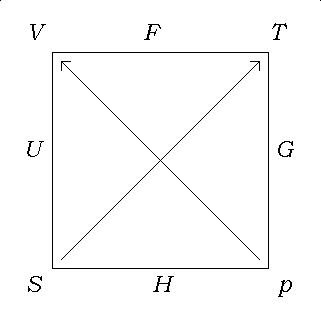
\includegraphics[width=0.5\textwidth]{potenciales}
\caption{Regla mnemotécnica para los potenciales termodinámicos}
\label{fig:potenciales}
\end{figure}
\subsection{Funciones de Massieu}
Las funciones de Massieu son las transformada de Legendre de la entropía, que podemos llamar entropías libres.
La primera es el potencial de Massieu
\begin{equation}
\begin{gathered}
\Phi = S[T,V,\{X_i\}] = S - \frac{U}{T}\\
d\Phi = -U d\frac{1}{T} + \frac{p}{T} dV + \frac{Y_i}{T} dX_i\\
d\Phi = \frac{U}{T^2} dT + \frac{p}{T} dV + \frac{Y_i}{T} dX_i
\end{gathered}
\end{equation}
Ese potencial lo podemos entender como
\begin{equation}
\Phi = - \frac{F}{T}
\end{equation}
Lo mismo podemos hacer con la energía libre de Gibbs, llamada entropía libre de Gibbs o potencial de Planck,
\begin{equation}
\begin{gathered}
\Xi = S[T,p,\{X_i\}] = S - \frac{U}{T} - \frac{p}{T} V = - \frac{G}{T} = \Phi - \frac{p}{T} V\\
d\Xi = -U d\frac{1}{T} - V d\frac{p}{T} + \frac{Y_i}{T} dX_i\\
d\Xi = \frac{U + p V}{T^2} dT - \frac{V}{T} dp + \frac{Y_i}{T} dY_i
\end{gathered}
\end{equation}
Estas funciones son útiles en mecánica estadística, ya que el logaritmo de la función de partición (por la constante de Boltzmann) es igual a la función de Massieu respectiva a la condición del sistema.
\section{Relaciones fundamentales}
En este apartado vamos a estudiar algunas consecuencias matemáticas de la teoría hasta ahora descripta.
Además vamos a considerar las funciones que debo tener de otras teorías para que la termodinámica funcione, una ecuación caracteristica o varias ecuaciones de estado y derivadas.
\subsection{Relaciones de Maxwell}
De la teoría de los diferenciales exactos podemos derivar que para cualquier función $f(x,y)$ con diferencial
\[df = \frac{\partial f}{\partial x} dx + \frac{\partial f}{\partial y} dy\]
se verifica que las derivadas segundas crusadas son iguales, es decir
\[\frac{\partial^2 f}{\partial x y} = \frac{\partial^2 f}{\partial y x}\]
Todo esto si el diferencial es exacto, es decir si
\[\oint df = 0\]
Podemos encontrar una relación por cada función de estado, que llamamos \emph{relaciones de Maxwell}.
\subsection{Relaciones materiales}
Definamos algunas propiedades materiales. El calor específico es igual la relación entre el cambio de temperatura y el calor entregado para ese cambio
\begin{equation}
C = \frac{\delta Q}{d T} = T \frac{dS}{dT}
\end{equation}
Si estamos a volumen constante, podemos encontrar que
\begin{equation}
C_v = \left.\frac{\partial U}{\partial T}\right|_V = T \left.\frac{\partial S}{\partial T}\right|_V
\label{eq:cv}
\end{equation}
Si la presión es constante $dp = 0$, debemos escribor $dV$ en función de la temperatura y la presión, encontrando
\[C_p = T \frac{dS}{dT} = T \frac{\partial S}{\partial T} + T \frac{\partial S}{\partial V} \frac{dV}{dT} = C_v + T \left.\frac{\partial S}{\partial V}\right|_T \left.\frac{\partial V}{\partial T}\right|_p\]
donde usamos una relación de Maxwell (de $dF$) para el segundo término
\[\left.\frac{\partial S}{\partial V}\right|_T = \left.\frac{\partial p}{\partial T}\right|_V\]
con lo que obtenemos
\[C_p = C_v + T \left.\frac{\partial p}{\partial T}\right|_V \left.\frac{\partial V}{\partial T}\right|_p = C_v + T V \alpha \left.\frac{\partial p}{\partial T}\right|_V\]
Ahí definimos el coeficiente de \emph{expansión térmica} como
\begin{equation}
\alpha = \frac{1}{V} \left.\frac{\partial V}{\partial T}\right|_p
\end{equation}
Para el último término usamos que $dV = 0$, ya que la derivada es a volumen constante, y de la expresión del diferencial $dV$ despejamos $\dfrac{dp}{dT}$, que es
\[ \left.\frac{\partial p}{\partial T}\right|_V = \frac{\partial_T V |_p}{\partial_p V|_T} = \frac{\alpha}{\beta_T}\]
donde se definió la \emph{compresibilidad isotérmica}
\begin{equation}
\beta_T = - \frac{1}{V} \left.\frac{\partial V}{\partial p}\right|_T
\end{equation}
con lo que finalmente nos queda
\begin{equation}
C_p = C_v + T V \frac{\alpha^2}{\beta_T}
\end{equation}
Si tenemos tres de las relaciones materiales podemos deducir las demás, en caso de tener una sola fase (si tenemos más fases, habrá tres por cada fase).
Y podemos a su vez conseguir una relación entre la compresibilidad isotérmica y la \emph{compresibilidad isoentrópica}
\begin{equation}
\beta_S = - \frac{1}{V} \left. \frac{\partial V}{\partial p}\right|_S
\end{equation}
que es
\begin{equation}
\beta_T = \beta_S + \frac{T V \alpha^2}{C_p}
\end{equation}
\subsection{Ecuaciones características}
Si experimentalmente o por otro método teórico encontramos uno de los potenciales respecto a sus variables naturales, la teoría de ecuaciones diferenciales exactos nos permite integrar sin ninguna necesidad de constantes de integración.
Sin embargo, si no tenemos el potencial en sus variables naturales, tendremos el problema de las constantes de integración, que se transforman en funciones desconocidas.
Por ejemplo si tenemos la función $F(T,V,\{X_i\})$ en sus variables, podemos encontrar
\begin{equation}
\begin{gathered}
p = - \left.\frac{\partial F}{\partial V}\right|_{T}\\
S = - \left.\frac{\partial F}{\partial T}\right|_{V}\\
\end{gathered}
\end{equation}
y las relaciones de Maxwell acordes
\begin{equation}
\left.\frac{\partial p}{\partial T}\right|_V = \left.\frac{\partial S}{\partial V}\right|_T
\end{equation}
Además sabemos que $U = F + TS$, se tiene
\begin{equation}
C_v = \left.\frac{\partial U}{\partial T}\right|_V = T \left.\frac{\partial^2 F}{\partial T^2}\right|_V
\end{equation}
Lo mismo podemos hacer para los demás potenciales
\begin{equation}
\begin{gathered}
S = - \left.\frac{\partial G}{\partial T}\right|_p\\
V = \left.\frac{\partial G}{\partial p}\right|_T\\
\frac{\partial S}{\partial V} = \frac{\partial V}{\partial T}\\
C_p = -T \frac{\partial^2 G}{\partial T^2}\\
\beta_T = - \frac{1}{V} \frac{\partial^2 G}{\partial p^2}
\end{gathered}
\end{equation}
\begin{equation}
\begin{gathered}
T = \left.\frac{\partial H}{\partial T}\right|_p\\
V = \left.\frac{\partial H}{\partial p}\right|_T\\
\left.\frac{\partial V}{\partial S}\right|_p = \left.\frac{\partial T}{\partial p}\right|_S\\
\beta_S = - \frac{1}{V} \frac{\partial^2 H}{\partial p^2}
\end{gathered}
\end{equation}
\subsection{Ecuaciones de estado}
Una ecuación de estado se llama a una relación
\begin{equation}
Y_i = Y_i(\{X_j\})
\end{equation}
es decir una variable intensiva en función de las extensivas.
Ejemplos de eso puede ser
\[p = p(U,V) = p(S,V)\]
\[T = T(S,V) = T(U,V)\]
En general para gases tenemos que
\[p = p(T,V,N)\]
donde eliminamos $S$ por $T$ usando una transformación de Legendre.
Tener una ecuación de estado no te da toda la información termodinámica, pero teniendo todas las posibles para un sistema es equivalente a tener una ecuación característica, o tener las tres propiedades materiales necesarias por fase.
Si tenemos $r$ componentes, hay $r + 2$ ecuaciones (asumiendo que no hay más parámetros extensivos que $S$, $V$ y $N_i$), que nos dan toda las información del sistema.
Pero de la relación de Gibbs-Durheim podemos eliminar una ecuación, obteniendo $r + 1$ grados de libertad (que se corresponde con las variables intensivas independientes).
\section{Equilibrio}
En este apartado vamos a estudiar las propiedades en el equilibrio, sea térmico, mecánico o de otra especie.
Para eso usamos que la entropía es extremal, en particular máxima, para dos sistemas $1$ y $2$, y además que es aditiva
\[ dS_T = dS_1 + dS_2 = \frac{\partial S_1}{\partial X^1_i} dX^1_i + \frac{\partial S_2}{\partial X^2_i} dX^2_i \geq 0\]
Consideremos transformaciones cuasiestacionarias, así tenemos definido en todo el proceso las variables (en caso de no ser transformaciones reversibles, siempre podemos construirnos una tranformación intermedia reversible, si sabemos el estado inicial y final).
Esto último determina que la desigualdad es una igualdad
\[\frac{\partial S_1}{\partial X^1_i} dX^1_i + \frac{\partial S_2}{\partial X^2_i} dX^2_i = 0\]
El cambio de una magnitud extensiva en un sistema es menos el cambio de la otra, y para convencernos de eso pensemos en la energía y la cantidad de partículas, o el volumen si hay un pistón movil entre los dos sistemas.
Eso nos lleva a concluir que
\begin{equation}
\frac{\partial S}{\partial X^1_i} = \frac{\partial S}{\partial X^2_i}
\end{equation}
que para substancias definidas por $T$, $p$ y $\mu$ indica que
\begin{equation}
\begin{gathered}
T_1 = T_2 \\
p_1 = p_2 \\
\mu_1 = \mu_2
\end{gathered}
\end{equation}
que son el equilibrio térmico, mecánico y químico respectivamente.
\subsection{Estabilidad}
En todo el análisis anterior usamos que la entropía es un extremo, pero nos falta observar que implica que además sea un máximo.
En general la forma del extremo determina la \emph{estabilidad} del sistema, y en este caso como es un máximo de entropía, y por lo tanto un mínimo de energía, los equilibrios van a ser \emph{estables}.
Como ya vimos el máximo de la entropía se escribe
\[d^2 S \leq 0\]
que implica que la función debe ser concava en un entorno del equilibrio.
De la teoría del análisis multifuncional sabemos que el desarrollo de Taylor a orden 2 corresponde a
\[ f(\textbf{x}) = f(\textbf{x}_0) + Df(\textbf{x}_0) (\textbf{x} - \textbf{x}_0) + (\textbf{x} - \textbf{x}_0)^{T} Hf(\textbf{x}_0) (\textbf{x} - \textbf{x}_0) + R(f, \textbf{x},\textbf{x}_0)\]
donde el primer orden dispone del diferencial o jacobiano de la función y el segundo orden corresponde al hessiano (que podemos pensar como un tensor de rango 2), más el resto de Taylor (que para funciones analíticas es simplemente seguir escribiendo ordenes superiores, que podemos pensar como tensores).
Si la función $f(\textbf{x})$ tiene un extremo el teorema de Taylor nos determina la positividad del hessiano.
Para un máximo el hessiano debe ser definido negativo, y para un mínimo debe ser definido positivo.
El criterio de Sylvester nos indica que una matriz es definida positiva si todos los menores tienen determinantes positivos, o definida positiva si todos los menores con dimensión k pares son negativos y los impares positivos.
En caso de al entropía, que es una función $S(U,V,\{X_i\})$, sabemos que debe ser máxima en el equilibrio, por lo que usando el criterio de Sylvester se llega a que
\begin{equation}
\begin{gathered}
\left.\frac{\partial^2 S}{\partial U^2}\right|_{V,X_i} \leq 0 \qquad
\left.\frac{\partial^2 S}{\partial V^2}\right|_{U,X_i} \leq 0\\
\frac{\partial^2 S}{\partial U^2} \frac{\partial^2 S}{\partial V^2} - \left(\frac{\partial^2 S}{\partial U \partial V}\right)^2 \geq 0
\end{gathered}
\end{equation}
Para más variables se extrapola de forma análoga, pensando en el criterio propuesto.
La primera relación la podemos escribir
\[\left.\frac{\partial^2 S}{\partial U^2}\right|_V = - \frac{1}{T^2} \left.\frac{\partial T}{\partial U}\right|_V = - \frac{1}{T^2 C_v} \leq 0\]
lo que nos lleva a
\begin{equation}
C_v \geq 0
\end{equation}
Para continuar nos conviene ver la energía $U$, que sabemos que debe ser un mínimo, es decir
\begin{equation}
\begin{gathered}
\frac{\partial^2 U}{\partial S^2} = \left.\frac{\partial T}{\partial S}\right|_V \geq 0 \qquad
\frac{\partial^2 U}{\partial V^2} = - \left.\frac{\partial P}{\partial V}\right|_S \geq 0\\
\frac{\partial^2 U}{\partial S^2} \frac{\partial^2 U}{\partial V^2} - \left(\frac{\partial U}{\partial S \partial V}\right)^2 \geq 0
\end{gathered}
\end{equation}
Para los potenciales podemos hacer el mismo proceso, recordando el cambio de signo de la variable que cambiamos, por lo que si para la energía respecto a la entropía es un minimo, el potencial respecto a la temperatura será un máximo.
\begin{equation}
\left.\frac{\partial^2 F}{\partial^2 T}\right. = \left.\frac{\partial S}{\partial V}\right|_V \leq 0 \qquad
\left. \frac{\partial^2 F}{\partial^2 V}\right. = \left.\frac{\partial p}{\partial V}\right|_T \geq 0
\end{equation}
\begin{equation}
\left.\frac{\partial^2 G}{\partial T^2}\right. = \left.\frac{\partial S}{\partial T}\right|_p \leq 0 \qquad
\left.\frac{\partial^2 G}{\partial p^2}\right. = \left.\frac{\partial V}{\partial p}\right|_T \leq 0
\end{equation}
\begin{equation}
\left.\frac{\partial^2 H}{\partial S^2}\right. = \left.\frac{\partial T}{\partial S}\right|_p \geq 0 \qquad
\left.\frac{\partial^2 H}{\partial p^2}\right. = \left.\frac{\partial V}{\partial p}\right|_S \leq 0
\end{equation}
De estas expresiones podemos deducir las condiciones para las propiedades materiales
\begin{equation}
\begin{gathered}
C_{V,p} \geq 0\\
\beta_{T,S} \geq 0\\
\alpha_{P,V} \geq 0
\end{gathered}
\end{equation}
Pero además si consideramos la siguiente idéntidad
\begin{equation}
\frac{\beta_S}{\beta_T} = \frac{C_V}{C_p}
\end{equation}
encontramos que
\begin{equation}
\beta_T \geq \beta_S \geq 0 \qquad C_p \geq C_V \geq 0
\end{equation}
Recordemos que todas estas igualdades encontradas en este apartado son propias de los estados de equilibrio estables.
Pueden no verificarse en equilibrios inestables o metaestables, como vamos a ver en el apartado de cambio de fases.
\subsection{Principio de Le Chatelier}
Este principio dictamina que cualquier inhomogeneadad de un sistema en equilibrio tenderá al sistema a otro nuevo equilibrio, volviendo a la homogeneidad.
Esto lo podemos deducir sabiendo que las relaciones materiales son positivas, ya que si agregamos calor al sistema o si lo comprimimos, la fluctuación se va esparciendo en virtud de la positividad de las constantes.
Pero también podemos deducir que el comportamiento del sistema frente a fluctuaciones de un parámetro intensivo $X^f$ cualquiera; el subscripto indica que es una fluctuación.
Para eso, tomemos dos subsistemas $1$ y $2$, tal que el sistema esté aislado.
El cambio del parámetro $Y$ del sistema $1$ va a ser
\[dY^f_2 = \frac{\partial Y_1}{\partial X_1} dX^f_1\]
además que altera al sistema $2$
\[ dY^f_2 = \frac{\partial Y_2}{\partial X_1} dX^f_1\]
Hasta ahora definimos los cambios debido a las fluctuaciones.
Pasemos a describir el cambio de la energía debido a las respuestas, que señalaremos con un superindice $r$
\[d(U + U^r) = (Y_1 - Y^r_1) dX^r_1 + (Y_2 - Y^r_2) dX^r_2 \leq 0 \]
donde usamos que la energía debe ser un mínimo.
La expresión de arriba puede llevar finalmente a
\[ d(U + U^r) = dY^f_1 dX^r_1 + dY^f_2 dX^r_2 \leq 0\]
Como los diferenciales son independientes, tenemos que
\[dY^f_1 dX^r_1 = \frac{\partial Y_1}{\partial X_1} dX^f_1 dX^r_1 \leq 0\]
\[dY^f_2 dX^r_2 = \frac{\partial Y_2}{\partial X_1} dX^f_1 dX^r_2 \leq 0\]
La primera desigualdad nos indica que
\begin{equation}
dX^f_1 dX^r_1 \leq 0
\end{equation}
La respuesta de la variable intensiva es contraria a la fluctuación, es decir el principio de Le Chatelieur.
La segunda desigualdad la podemos trabajar usando una relación de Maxwell derivada de la energía
\[ \frac{\partial Y_2}{\partial X_1} = \frac{\partial Y_1}{\partial X_2}\]
en la forma
\[dX^f_1 \frac{\partial Y_1}{\partial X^2} dX^r_2 \leq 0.\]
Si multiplicamos a ambos lados por $\partial_{X_1} Y_1$ que sabemos que es positiva obtenemos
\[\frac{\partial Y_1}{\partial X_1} dX^f_1 \frac{\partial Y_1}{\partial X_2} dX^r_2 \leq 0\]
que es lo mismo que
\begin{equation}
dY^f_1 dY^r_1 \leq 0
\end{equation}
Nuevamente encontramos que la fluctuación del parámetro intensivo genera una respuesta contraria, en línea con el principio de Le Chatelieur.
\section{Cambio de fases}
En este apartado vamos a discutir el equilibrio y transición de fase
Toda transición de fase está caracterizada por una perdida de estabilidad de la substancia analizada en el sistema.
La fluctuaciones se encargaran de que la substancia esté en una fase u otra.
Las transiciones de fase se clasifican en \emph{primer orden} y \emph{segundo orden}, la primera tiene un calor latente y la segunda en general se llaman transiciones continuas, caracterizadas por una suceptibilidad (derivada segunda de la ecuación caracteristica) divergente.
Las transiciones de primer orden tienen además la particularidad de estar caracterizadas por la existencia de dos mínimos del potencial, separados por una barrera, mientras que las de segundo orden suceden en un sólo punto del espacio de configuraciones termodinámico (y por ello se denominan \emph{fenómenos críticos}).
Para las transiciones de primer orden podemos definir al calor latente como
\begin{equation}
l = T \Delta s
\end{equation}
siendo $\Delta s$ la diferencia de entropía molar entre las fases.
Como estamos hablando de una transiciones que ocurren a temperatura constante (y las fluctuaciones son debidas a alguna otra variable), trabajaremos con las energías libres.
En esas energías libres se observa la existencia de dos mínimos, uno más estable que otro (a menor energía libre, más estable).
Como la transición se efectúa a temperatura constante, debe haber un cambio de entropía (que lo tratamos de forma molar, para eliminarnos la cantidad de materia).
\subsection{Coexistencia de fases}
En los diagramas termodinámicos podemos encontrar curvas de coexistencia de fase, usando que como es un equilibrio entre dos especies.
Es decir
\[\mu_{1} = \mu_{2}\]
que es igual a la energía libre de Gibbs por mol de cada fase.
Tratarermos coexistencia de fases con presión y temperatura, ya que los casos que nos preocupan hay variaciones importantes de volumen molar.
Elijamos dos estados $A$ y $A'$ sobre la curva de coexistencia, pero de diferentes fases, lo mismo con $B$ y $B'$.
La diferencia de presión entre $A$ y $B$ la consideramos
\[p_B - p_A = dP\]
y lo mismo para la temperatura
\[T_B - T_A = dT\]
La curva de coexistencia tiene de pendiente $dp/dT$ en un diagrama $p-T$
Como estoy en un equilibrio de fases
\[\mu_A = \mu_A' \qquad \mu_B = \mu_B'\]
por lo que
\[\mu_B - \mu_A = \mu_B' - \mu_A'\]
y usando que $\mu$ es la energía libre por mol
\[\mu_B - \mu_A = -s dT + v dp = \mu_B' - \mu_A' = -s' dT + v' dp\]
de lo que deducimos finalmente
\begin{equation}
\frac{dp}{dT} = \frac{s' - s}{v' - v} = \frac{\Delta s}{\Delta v} = \frac{l}{T \Delta v}
\label{eq:clausius_clayperon}
\end{equation}
Esta es la ecuación de Clayperon, que determina la pendiente de las curvas de coexistencia, y además tiene embuido el principio de Le Chatelieur.
\[d\mu = \frac{V} dp + S dT\]
Como ya dijimos vamos a trabajar con presión y temperatura, pero en particular vamos a buscar cambios de fases a temperatura constante.
\subsection{Isotermas inestables}
Aunque las transiciones de primer orden las podemos entender como la existencia de varios minimos en la energía libre, podemos también encontrar casos de isotermas inestables, en particular en un diagrama $p-V$.
A saber, la segunda ley determina que
\[ \frac{\partial p}{\partial V}_T \leq 0\]
que en algunas ecuaciones de estado para gases no se cumple.
En general el proceso ocurre debido a que la ecuación de estado está derivada de ciertas hipótesis mecánicas sobre la substacia, como ser el gas ideal o de Van Der Waals, pero que algunas de las hipótesis se violan en la inestabilidad.
Al haber un estado inestable, y tener un cambio de fases gas a líquido, se pierde la hipótesis de homogeneadad, por lo que esa parte de la ecuación fundamental (o de estado) debe ser \emph{arreglada}.
Como estamos en un cambio de fases, debemos considerar el potencial químico entre dos estados sobre la isoterma, el cual podemos calcular por medio de la relación de Gibbs Durheim
\begin{equation}
\mu_B - \mu_A = \int^B_A v dP
\label{eq:isoterma_eq_fase}
\end{equation}
donde la constante de integración dependiente de la temperatura se eliminó al calcular variaciones del potencial químico.
Definido el potencial químico, la energía libre de Gibbs molar, y sabiendo que la presión en función del volumen tiene derivada positiva en algún intervalo, podemos deducir que el volumen respecto a la presión va a ser una función multivaluada.
De esta forma al integrar el volumen, la energía libre también será multivaluada, llevando a una contradicción.
Para salvar la contradicción, exigimos que el potencial químico en todo ese intervalo sea constante, propio de una curva de coexistencia de fases, por lo que la integral de \ref{eq:isoterma_eq_fase} esa nula
\begin{equation}
\int^B_A v dp = 0
\label{eq:regla_maxwell}
\end{equation}
que se llama regla de Maxwell, que para una isoterma oscilante exige areas iguales.
Para un gas de Van der Waals la forma de la curva de coexistencia será una recta horizontal generando areas iguales.
Recién cuando truncamos la isoterma con la regla de Maxwell tenemos una curva físicamente posible.
Esa curva crea un cambio brusco de $v(p)$, del volumen molar, por lo que también produce un cambio brusco de la entropía molar.
Como la entropía es una función de estado podemos integrarla con
\[ \Delta s = \int \left.\frac{\partial s}{\partial v}\right|_T dv = \int \left.\frac{\partial p}{\partial T}\right|_V dv\]
sobre la curva ficticia.
En cambio de entropía corresponde a un calor latente intercambiado.
Esto conlleva también un cambio de la energía interna molar, ya que
\[ \Delta u = T \Delta s - p \Delta v\]
Si unimos los extremos de las rectas de coexistencia según la regla de Maxwell obtenemos una curva tipo parabóla, que separa el diagrama $p-v$ en dos fases, gaseosa y líquido más gas.
La fracción de gas y líquido en la zona de coexistencia viene dado por la regla de la palanca, que corresponde a asumir que existe una sóla substancia con volumen $V = N v$, divida en dos subsistemas con volumenes $V_G = N x_g v_G$ y $V_L = N x_L v_L$, siendo $x_i$ la fracción molar ($\sum x_i = 1$).
Finalmente la regla queda
\begin{equation}
x_L = \frac{v_G - v}{v_g - v_L} = 1 - x_G
\end{equation}
La inestabilidad de un potencial genérico en función de sus variables $X_j$ lo podemos corregir uniendo con una línea recta los dos mínimos separados por una barrera, como vemos en la figura \ref{fig:fase_potencial}
\begin{figure}[H]
\centering
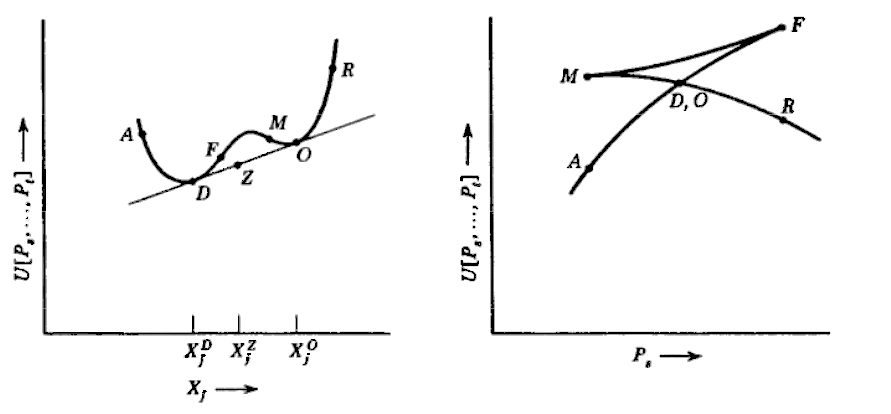
\includegraphics[width=0.5\textwidth]{fase_potencial}
\caption{Potencial generalizado en un caso de perdida de estabilidad, además de la correción con el método de Maxwell}
\label{fig:fase_potencial}
\end{figure}
La línea entre $D$ y $O$ se consigue exiguiendo potencial químico constante, como ya hicimos previamente para el caso isotérmico con el potencial de Gibbs..
\subsection{Regla de las fases de Gibbs}
Imaginemos que tenemos $R$ componentes en un equilibrio de fase.
Ya sabemos $R$ componentes diferentes implica que haya $R + 1$ variables
Consideremos que hay $N$ fases, por lo que las variables independientes de cada potencial químico van a ser $2 + M(r - 1)$ ($T$, $p$ y las fracciones molares).
Pero a su vez existen $r(M - 1)$ ecuaciones dadas por el equilibrio de fase, que corresponde a la igualdad entre potenciales químicos.
Esto nos dice que los grados de libertad que vamos a tener son
\begin{equation}
f = 2 + M(r - 1) - r(M - 1) = r - M + 2
\label{eq:regla_gibbs_fase}
\end{equation}
ecuación que se denomina regla de Gibbs de las fases.
De ahí podemos deducir que si tenemos un sólo componente, el punto triple no tiene grados de libertado posibles, por lo que es un único estado y además si hay dos fases para una componente tenemos una curva donde hay un sólo grado de libertad.
Si se tiene más grados se pasará a tener una superficie de coexistencia de fases.
\section{Tercer principio}
Un agregado final debido a Nerst, que se puede entender solamente en el contexto de la mecánica cuántica, es la tercera ley de la Termodinámica
\begin{law}[Mínimo de la entropía]
La entropía de un sistema tiende a una constante positiva al hacer nula la temperatura. Es decir
\[\displaystyle\lim_{T \to 0} S = S_0 \geq 0\]
Este valor corresponde al mínimo de entropía.
\end{law}
De esta ley, junto con la segunda ley, podemos deducir que no es posible alcanzar la temperatura $T = 0$ llamado cero absoluto.
La constante positiva podemos entenderla como la entropía remanente, debido a la degeneración del estado fundamental, que sólo se puede comprender entiendiendo la cuántica.
\section{Gases reales e ideales}
En este apartado vamos a presentar algunas ecuaciones de estado para gases, ideal o real, derivadas de principios básicos de la mecánica estadística.

\subsection{Gas ideal}
Podemos deducir de algunos resultados experimentales o simplemente deduciendola de la mecánica estadística: para un gas ideal, es decir sin interacciones entre partículas tenemos que
\begin{equation}
p V = n R T
    \label{eq:gas_ideal_estado}
\end{equation}
que corresponde al una ecuación de estado $p = p(V, n, T)$, con $n$ la cantidad de moles de substacia.
De esta forma la transformaciones isocóricas y isométricas son triviales, mientras que las transformaciones isotérmicas
\begin{equation}
    p = \frac{T}{v}
\end{equation}
son hipérboles en el plano $p-V$, como se ve en la figura \ref{fig:gas_ideal_isotermas}.
\begin{figure}[H]
    \centering
    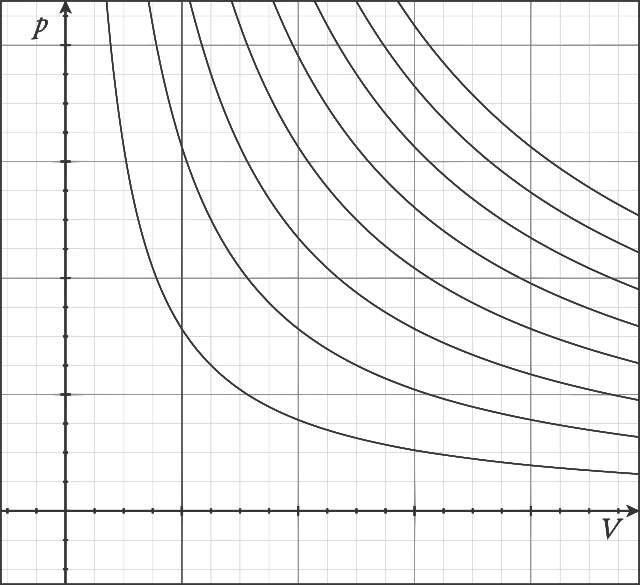
\includegraphics[width=0.4\textwidth]{gas_ideal_isotermas}
    \caption{Isotermas de un gas ideal con unidades arbitrarias}
    \label{fig:gas_ideal_isotermas}
\end{figure}

Interesante es que debido a la ecuación de estado, la energía $U$ no depende del volumen, ya que si tomamos el diferencial de entroía 
\[  dS = \left.\frac{\partial S}{\partial T}\right|_V dT + \left.\frac{\partial U}{\partial V}\right|_T dV\]
y lo reemplazo en la expresión de la primera/segunda ley
\[ dU = T \left.\frac{\partial S}{\partial T}\right|_V dT + \left( T \left.\frac{\partial S}{\partial V}\right|_T - p \right) = C_v dT + \left( T \left.\frac{\partial p}{\partial T}\right|_V - p \right) = C_v dT \]
es decir que la energía interna para un gas ideal es simplemente
\begin{equation}
    dU = C_v dT
    \label{eq:gas_ideal_energia}
\end{equation}

Experimentalmente (y de la mecánica estadística) se encuentra que el calor específico es constante con la temperatura y que además vale
\begin{equation}
    C_v = \frac{3}{2} N k_B
    \label{eq:gas_ideal_cv}
\end{equation}
Con esto tenemos el gas ideal caracterizado, porque podemos deducir la energía interna
\begin{equation}
    U = \frac{3}{2} N k_B T
\end{equation}
donde aparece la \emph{equipartición de la energía} en forma de tres grados de libertad con $\frac{N k_B T}{2}$ energía, y también podemos encontrar la entropía
\begin{equation}
    S = C_v \ln\left(\frac{T}{T_0}\right) + N K \ln\left(\frac{V}{V_0}\right)
\end{equation}
A partir de la expresión de la entropía podemos deducir la funciona de una transformación adiabática, usando que la entropía $S = cte$,

\begin{equation}
    V T^{\frac{C_v}{N k_B}} = c \qquad T V^{\frac{N k_B}{C_v}} = c
\end{equation}
que se puede llevar a
\begin{equation}
    p V^{1 + \frac{C_v}{N k_B}} = p V^{\frac{C_v + N k_B}{C_v}} = p V^{\gamma} = c
\end{equation}
donde también podemos deducir que
\begin{equation}
    C_p - C_v = N k_B
\end{equation}
por lo que 
\begin{equation}
    \gamma = \frac{C_p}{C_v}
\end{equation}
que para un gas ideal monoatómico es igual a $\gamma \dfrac{3}{2}$.
Esa relación la diferencia de una isoterma, que sería de la forma de una adiabática pero con $\gamma = 1$, que sólo es posible de obtener si el gas tiene 2 grados de libertad (como un gas en dos dimensiones).

\subsection{Gas de Van der Waals}

La primer teoría exitosa de los gases reales fue la propuesta por Van Der Waals, proponiendo la existencia del volumen excluido, que corresponde al volumen de cada partícula de gas, y a la iteracción por choques entre partículas, que trató a primer orden.
De esta forma llegamos a que 
\begin{equation}
\left(p + \frac{a N^2}{V^2}\right)(V- b N) = N k_B T
\label{eq:vanderwalls}
\end{equation}
que podemos escribir de la siguiente forma
\begin{equation}
p = \frac{R T}{v - b} - \frac{a}{v^2}
\label{eq:vanderwalls_intensivo}
\end{equation}
La ecuación de Van der Waals es exitosa en describir cualitativamente el comportamiento de los gases reales, sin producir comportamientos físicamente absurdos, pero cuantitavamente varía mucho dependiendo de la elección de los parámetros $b$ y $a$.

Veamos las isotermas, que las graficamos en la figura \ref{fig:gases_vdw_isotermas}
\begin{figure}[H]
    \centering
    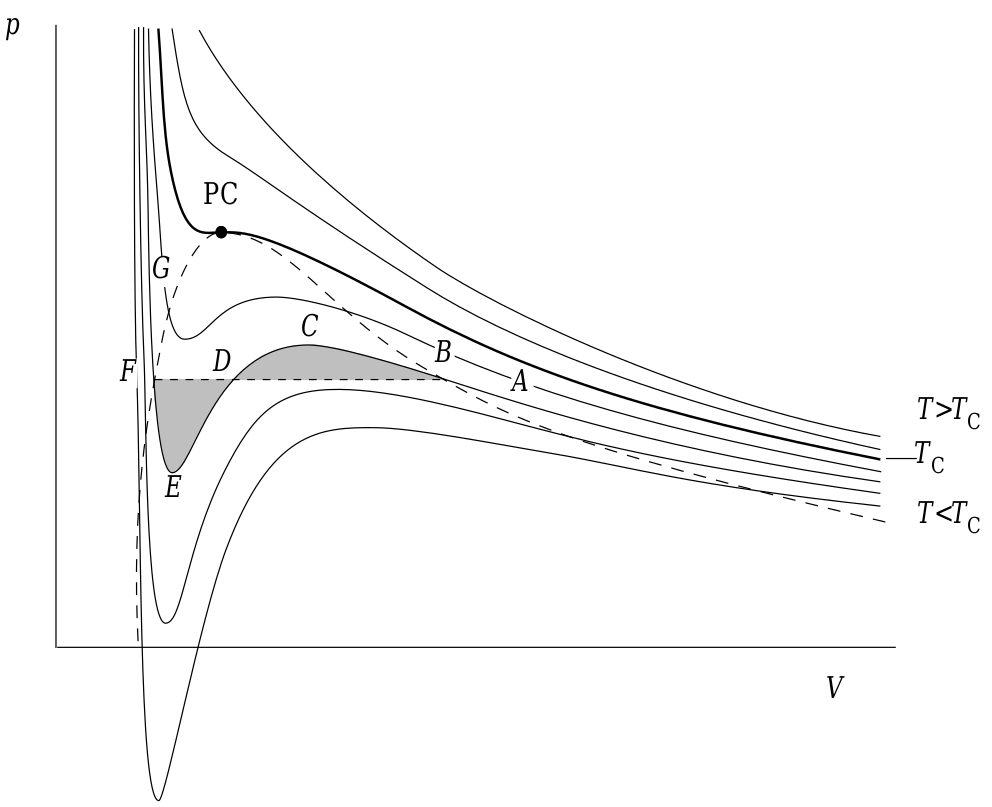
\includegraphics[width=0.5\textwidth]{gases_vdw_isotermas}
    \caption{Diagrama p-V con isotermas, adimensionalizadas, del gase de Van der Waals, más el punto crítico y la zona de coexistencia}
    \label{fig:gases_vdw_isotermas}
\end{figure}

En esa figura se observa que dentro de la zona demarcada por la curva punteada existe una oscilación que no tiene correlato físico, ya que es inestable.
En esa zona se produce un cambio de fase, y se arregla con la regla de Maxwell, recta que está marcada con el sombreado en una de las oscilaciones.

Mientras el punto crítico nos permite definir una temperatura, volumen y presión y adimensionalizar la ecuación de Van der Waals.
En el punto crítico tenemos que

\begin{equation}
    \left.\frac{\partial p}{\partial V}\right|_{T_c} = 0 \qquad \left.\frac{\partial^2 p}{\partial V^2}\right|_{T_c} = 0
\end{equation}

La primer condición y la segunda condición implican que
\begin{equation}
    v^3 = \frac{2 a}{k_B T_c} (v - b)^2 \qquad 3 v^2 = \frac{4 a}{k_B T_c} (v - b)
\end{equation}
donde usamos la expresión intensiva de la ecuación de Van der Waals y llevamos todo a una expresión simplificada.
Dividimos una por otra y obtenemos que
\[ \frac{1}{2} v = \frac{1}{2} (v - b) \]
lo que es lo mismo que el volumen crítico es igual
\begin{equation}
    v_c = 3 b
\end{equation}
Ahora despejamos la temperatura crítica por la constante de Boltzmann de la derivada segunda tenemos
\begin{equation}
    k_b T_C = \frac{8}{27} \frac{a}{b}
\end{equation}
De esta forma reemplazando la temperatura crítica y el volumen crítico en la ecuación de Van der Waals tengo la presión crítica

\begin{equation}
    p_C = \frac{k_B T_C}{v_C - b}  - \frac{a}{v^2_C} = \frac{1}{9} \frac{a}{b^2} \left(\frac{4}{3} - 1\right)
\end{equation}
Ahora si elijo variables $v = v' v_c$, $p = p' p_c$ y $T = t' T_c$ y las reemplazo en la ecuación de Van der Waals
\[ \left(p' p_c + \frac{a}{v'^2 v^2_c}\right) (v' v - b) = k_B T t' \] 
que termina resultando en
\begin{equation}
    \left(p' + \frac{3}{v'^2}\right)(3 v' - 1) = 8 t'
    \label{eq:gases_estados_correspondientes}
\end{equation}
que es una relación independiente de la substancia llamada ley de los estados correspondiente, que se verifica muy bien al adimensionalizar con el valor crítico cada gas.

\subsection{Ecuación del Virial}

Para completar la descripción de gases reales existe una ecuación de estado escrita como una serie, con cada término con significado físico
\begin{equation}
p v = RT \left( 1 + \sum_{i = 1} \frac{A_i}{v^i}\right)
\end{equation}
con cada coeficiente función solamente de la temperatura, y representa aspectos de las interacciones entre moléculas.
Esa expresión se denomina ecuación del estado virial.

\section{Motores térmicos}

\section{Introducción a la mecánica estadística}


\chapter{Mecánica cuántica}

\section{Introducción}
 La mecánica cuántica se encarga de la descripción del mundo microscópico, en general en escala atómica y subatómica, describiendo para eso la materia y la interacción con la radiación.
 Vamos a ver que muchas conclusiones de la mecánica cuántica chocan con nuestra intuición física, aunque no existe ningún argumento que nos asegure que se pueda extrapolar el pensamiento clásico o macroscópico a la escala que trabaja la cuántica.
 A principio del siglo XX se pudo refinar las experiencias sobre la materia, además del incipiente conocimiento de la teoría electromagnética, llegando a tratar directamente en la escala atómica.
 Varias experiencias no encuentran explicación plausible en la mecánica y electromagnetismo clásico, además de que no se podían entender la notable estabilidad del núcleo atómico.
 
 En todo el siglo XX se fue construyendo a partir del trabajo laborioso de varios brillantes científicos, que tuvieron que desechar algunos cimientos básicos de la física hasta ese momento.
 Lograron, empero, un edificio intelectual muy poderoso, que en la práctica resolvió todas los problemas a la que fue aplicado, y constituye una de las teorías con mayores aplicaciones teóricas y experimentales.
 
 Sin embargo la mecánica cuántica sufre desde sus inicios de una contradicción importante: la interpretación está desligada de la teoría. Debido a eso, no hay ninguna interpretación aceptada totalmente, y además esto conlleva a tener puntos oscuros en el proceder físico, como se el proceso de medición.
 
\section{Desarrollos históricos}

\subsection{Teoría atómica}
La naturaleza atómica y \emph{cuantizada} de la materia no se aceptó hasta empezado el siglo XX, cuando teorías como el movimiento browniano (explicado por Einstein en 1905) basados en la teoría cinética (propuesta por Joule y Boltzmann en 1860) lograron explicar muchisimas experiencias y además eran consistentes con los experimentos.

\subsubsection{Modelo de Thompson}
El primer modelo atómico, además del átomo de Democrito, fue propuesto por J. J. Thompson, que en sus experiencias con rayos catódicos fue capaz de encontrar una partícula con carga negativa con una relación masa a carga de $9.56 \times 10^8 C/g$.

La experiencia de rayos catódicos consiste en tener un tubo con un gas a una presión muy baja y dos electrodos, un ánodo y un cátodo.
Al disponer una diferencia de potencial en el orden de los $kV$, Thompson descubrió que existe una descarga del cátodo (que corresponde donde debería estar la carga negativa, y le dan el nombre al fenómeno) al ánodo, y además descubrió que dicha descarga tenía identidad corcupular, al tener un momento lineal asociado. 
Thompson llamó electrón a la partícula asociada a esos rayos, y construyó el modelo atómico del budin de pasa de uvas: como la materia es neutra, los electrones deben estar inmersos en una subtancia con carga positiva, con posibilidad de vibrar para generar radiación electromagnética y de ser arrancados para ser rayos catódicos.

Millikan con sus experimentos logró medir la carga del electrón, que vale 
\begin{equation}
 e = 1.603 \times 10^{-19} C
\end{equation}
y además sucesivos experimentos no pudieron determinar la existencia de una partícula con carga positiva en el átomo, verificando aún más la teoría de Thompson.

\subsubsection{Modelo de Rutherford}
Rutherford, con sus colaboradores Geiger y Marsden, analizaron al dispersión de partículas $\alpha$ al ser colicionadas con una lámina fina de metal.
Ellos buscaban confirmar el modelo de Thompson, sabiendo que la dispersión debería seguir una ley conocida para el metal en cuestión (ya que está determinado el número de electrones por experiencias por difracción de rayos X).
Además, Rutherford despreció la interacción con los electrones del modelo de Thompson, ya que al hacer las cuentas observó que se debían dispersar partes por mil de radian, ángulo para el cual no tenía capacidad de resolución.

Rutherford encontró que para ángulos pequeños la dispersión debido al modelo de Thompson funcionaba muy bien, pero encontró que había partículas que se dispersaban hasta 90$^\circ$.
Este hecho no se puede resolver ni explicar con el modelo de Thompson, por lo que Rutherford propone el modelo planetario: la carga positiva se encuentra concentrada en una pequeña región del espacio con los electrones orbitando.

Esa pequeña región del espacio la encontró Rutherford usando la ley de dispersión derivada de su modelo (en unidades cgs)

\begin{equation}
 \frac{\mathrm{d}\sigma}{\mathrm{d}\Omega} = \left(\frac{Q Z_2 e}{4 E_0}\right)^2 \frac{1}{\sin^4\left(\frac{\theta}{2} \right)}
\end{equation}

donde $Q$ y $E_0$ son la carga y la energía de la partícula dispersada, $Z$ es el número de electrones del átomo.
Observó de esta forma que el radio del núcleo es del orden de $10^{-12}$ cm, mientras que ya se sabía que el radio del átomo era de $10^{-8}$ cm, lo que determina que las propiedades químicas sólo depende de la distribución de electrones.

Este modelo tiene varias fallas de estabilidad, ya que los electrones orbitando según la teoría clásica de electromagnetismo deberían radiar al estar acelerados.

Para eso Bohr propuso fenomenológicamente su modelo atómico.

\subsubsection{Modelo de Bohr}

La inestabilidad intríseca, hallada con la teoría clásica, del modelo de Rutherford llevo a Bohr a proponer su teoría en 1913, con el mérito de explicar el espectro de radiación de algunos átomos.
Después la teoría de Bohr fue perfeccionada hasta llegar a la mecánica cuántica antigua, que finalmente fue sobrepasada por el formalismo que vamos a explicar más adelante.

El espectro de los átomos, ya observados en el siglo XIX, a diferencia de la radiación térmica, es discreta y cada longitud de onda se denomina \emph{línea}.
La primera relación de origen experimental para las líneas del hidrógeno fue dada por Balmer, con la siguiente expresión
\begin{equation}
    \frac{1}{\lambda_{2,n}} = R_H \left(\frac{1}{2^2} - \frac{1}{n^2}\right) \qquad n = 3, 5, 7
\end{equation}
con la constante de Rydberg para el hidrógeno 
\begin{equation}
    R_H = 109677,575\pm0,012 \,\text{cm}^-1
\end{equation}
Posteriormente Rydberg generalizó todas las series
\begin{equation}
    \frac{1}{\lambda_{m,n}} = R_H \left(\frac{1}{m^2} - \frac{1}{n^2}\right) \qquad m \in \mathbb{N},\; n = m + 1,\,m + 2,\,m + 3,\dots
\end{equation}
y si $m = 1$ son las series de Lyman, $m = 2$ la de Balmer, $m = 3, 4$ y $5$ son las de Paschen, Brackett y Pfund respectivamente.

Para poder explicar esto, Bohr propne que el electrón del hidrógeno está atado a la interacción columbiana con el núcleo, pero las orbitas clásicas pasan a estar discretizadas, considerando que el momento angular $L = n\hbar = n h/2\pi$.
Además considera que aún estando acelerado clásicamente, no irradia si está en alguna orbita discretizada o \emph{permitida}.

Como las orbitas permitidas son discretas, el electrón sólo puede recibir la energía suficiente para pasar a otra orbita, y finalmente radiarla en forma de un fotón, con frecuencia $\nu = \Delta E / h$

Si aplicamos las ideas de Bohr, tenemos que la fuerza centrípeta debe ser igual a la fuerza electromagnética (considerando el núcleo quieto o con masa casi infinita)
\[ \frac{m_e v^2}{r} = \frac{Z e^2}{r^2} \]
y como la fuerza es central, el momento angular se conserva
\[ L = m_e v r = cte.\]
Si remplazamos el momento angular en la fuerza centrípeta
\[ Z e^2 = \frac{L^2}{m_e r}\]
es decir
\[ r = \frac{L^2}{m_e Z e^2}\]
De esta forma los radios permitidos serán los que tengan $L = n\hbar$
\begin{equation}
    r_n = \frac{n^2 \hbar^2}{m_e Z e^2}
\end{equation}
También la velocidad angular del electrón está cuantificada
\begin{equation}
    v_n = \frac{n\hbar}{m_e r_n} = \frac{Z}{n} \alpha c
\end{equation}
donde definimos la constante $\alpha$ como de la estructura fina
\begin{equation}
    \alpha = \frac{e^2}{\hbar c} = 7,297 \times 10^{-3} \approx \frac{1}{137}
\end{equation}

La velocidad más pequeña posible con este análisis es mucho menor que la velocidad de la luz, porque no cometimos un error grosero en este análisis.

Ahora calculemos la energía del electrón
\[ E_n = T_n + V_n = \frac{1}{2} m_e v^2_n - \frac{Z e^2}{r_n} = - \frac{1}{2} m_e v^2_n\]
que finalmente es igual a
\begin{equation}
    E_n = -\frac{m_e}{2n^2}\left(\frac{Z e^2}{\hbar}\right)^2 = \frac{Z}{n^2} E_1
\end{equation}
con la energía del fundamental
\begin{equation}
    E_1 = - \frac{1}{2} \frac{m_e e^4}{\hbar^2} = -\frac{1}{2} m_e c^2 \alpha^2 = -13,6\,\text{eV}
\end{equation}
Con esta energía cuantizada, y sabiendo que el fotón debido a la transición entre dos energías diferentes $\nu = \Delta E / h$, Bohr predijo de forma correcta las series del átomo de hidrógeno y del helio ionizado, es decir átomos con un sólo electrón.

Posteriormente Sommerfeld y Wilson generalizaron las ideas de Planck y Bohr proponiendo que para un sistema cuántico con coordenada ciclica $q$ y su momento conjugado $p$ se verifica que
\begin{equation}
    \oint p dq = n h \qquad n \in \mathbb{N}
\end{equation}
relación para la cual se demuestra que para un oscilador armónico observamos la cuantificación de la energía y además para orbitas circulares y elipticas la energías de Bohr.

\subsection{Cuerpo negro}
La radiación de cuerpo negro consiste en un cuerpo en equilibrio térmico con la radiación, con el énfasis en la forma de la radiación.
Para eso sabemos de la mecánica estadística que la presión de radiación es
\[ p = \frac{u}{3} \]
donde $u$ es la densidad de energía. De la ecuación diferencial para la energía interna deducimos
\[dU = d(u V) = V du + u dV = T dS - p dV = T d(s V) - \frac{u}{3} dV = T s dV + T V ds - \frac{u}{3} dV\]
y si usamos que $u(T)$ y $s(T)$, ya que no hay otra variable termodinámica, llegamos a
\[ \left( \frac{\mathrm{d} u}{\mathrm{d} T} - T \frac{\mathrm{d} s}{\mathrm{d} T} \right) dT = \left(s T - \frac{4}{3} u \right) \frac{dV}{V}.\]

Como los diferenciales son independientes, ambos términos deben ser nulos simultáneamente. 
Al hacerlos llegamos a que

\begin{equation}
\begin{gathered}
 s = \frac{4}{3} \sigma T^3\\
 u = \sigma T^4
\end{gathered}
\end{equation}
que corresponde a la ley de Stefan-Boltzmann, con la constante 
\begin{equation}
\sigma = 5,67\times 10^{-8} \rm\textstyle \frac{W}{m^2 \cdot K^4} 
\end{equation}

Si pensamos a la radiación como muchas ondas planas incoherentes, podemos llegar a encontrar una función de distribución que dependa de la frecuencia (o longitud de onda) de la radiación electromagnética y de la temperatura, que nos determine la energía por unidad de volumen.

Para encontrar la energía por volumen consideremos una caja en equilibrio térmico interno con la radiación, aislada (esto no hace perder la validez para otras experiencias, pero permite simplificar el razonamiento).
Como es un sistema cerrado podemos contabilizar los modos de onda planos, sumandolos con una sumatoria, que van a determinar la energía.

La energía debido a cada longitud de onda viene dada por la energía de cada onda, que la teoría electromagnética nos dice que es
\begin{equation}
 u = c \varepsilon E^2
\end{equation}
y por la definición de cuerpo negro
\begin{definition}
    Un cuerpo negro es tal que toda la energía en forma de radiación incidente es irradiada, sin absorber nada.
\end{definition}
Con esto queda claro que simplemente debemos sumar todas las longitudes de onda incidentes y irradiadas para determinar la energía en función de la temperatura.

Si vamos a contar modos de ondas, primero las sumo y luego debo pasar al continuo, teniendo en cuenta que el número de onda está dado por 
\[ k = \frac{2 \pi}{L} n \]
donde se dispuso las condiciones de contorno adecuadas.
Si además estamos buscando la densidad de estados debemos eliminar el volumen por lo que la integral pasa a ser
\[ \frac{1}{V} \sum_N \to \frac{1}{V} \int \frac{\mathrm{d}^3k}{(2\pi)^3}\]
y si usamos que el medio es isótropo podemos integrar en esféricas con $\mathrm{d}^3k = 4\pi k^3 \mathrm{d}k$.

Finalmente si consideramos la polarización de las ondas electromagnéticas e integramos en frecuencia en vez de número de ondas (recordando que $k = \frac{\nu}{c}$) tenemos que
\begin{equation}
 u = \frac{1}{\pi^2 c^3} \int^\infty_0 \nu^2 f(\nu,T) d\nu
\end{equation}

Nos queda saber la forma de la función de $f(\nu,T)$.

Existían dos teorías que trataban de explicar las mediciones, la ley de Wien
\begin{equation}
    f = c' \nu e^{-c\;\nu \beta}
\end{equation}
donde la constante $c$ se observó constante y con unidades de energía por tiempo (por lo que la derivada tiene unidades de energía) y además $\beta = \frac{1}{k_B T}$, la temperatura de Boltzmann.
Este modelo corresponde a una deducción experimental.

La otra posibilidad era la idea de Rayleigh-Jeans, que correspondía a un intento teórico usando la realidad ondulatoria de la radiación.

Experimentalmente ambos funcionaban, pero Rayleigh-Jeans divergía para frecuencias altas, lo que se llamó la catástrofe del ultravioleta, por lo que no es explicable desde la mecánica clásica la radiación de cuerpo negro. 

Para eso Planck propone el siguiente desarrollo, usando la la mecánica estadística: 
como estamos en equilibrio térmico, la probabilidad de encontrar el sistema con energía $\varepsilon$ es 
\[ P(\varepsilon) = e^{-\beta \varepsilon}\]
con lo que el valor medio de la energía va a ser
\[ \langle E \rangle = \frac{\int \varepsilon e^{-\beta \varepsilon} d\varepsilon}{\int e^{-\beta \varepsilon'} d\varepsilon'} = \beta \int \varepsilon e^{-\beta \varepsilon} d\varepsilon\]
donde la integral en el numerador se denomina función de partición $Z$, la cual normaliza la probabilidad al ser una suma sobre todos los estados.
A partir de acá, Planck propone que la energía de cada oscilador es un múltiplo de $h\nu$, constante que denominó con su nombre, con valor (actual) de
\begin{equation}
h = 6,626 \times 10^{-27}\,\text{erg}\,\text{s}.
\end{equation}
Sabiendo que la energía de cada oscilador estaba \emph{cuantizada} o discretizada, la función de partición pasa a ser
\[ Z = \sum^\infty_{n = 0} e^{-n \beta \varepsilon} = \frac{1}{1 - e^{-\beta \varepsilon}}\]
donde usamos que el equispaciado da una energía muy pequeña respecto a la cantidad de osciladores, teniendo una serie geométrica. 
Además de la mecánica estadística podemos deducir que la energía libre es
\begin{equation}
    \langle E \rangle = - \frac{\partial}{\partial \beta} \ln(Z)
\end{equation}
por lo que finalmente nos queda que que la densidad de energía con la proposición de Planck es
\begin{equation}
  u = \frac{1}{\pi^2 c^3} \int^\infty_0 \frac{h \nu^3}{e^{\beta h \nu} - 1} d\nu
\end{equation}
que se llama ley de Planck.
Si resolvemos la integral, llegamos a la ley  de Stefan-Boltzmann, con la constante igual 
\begin{equation}
\sigma=\frac{2\pi^5 k^4}{15c^2h^3}= 5.6704 \cdot 10^{-8}\; \rm\frac {W}{m^2 \cdot K^4}
\end{equation}
\subsection{Efecto fotoeléctrico}

El efecto fotoeléctrico se observa a tener un tubo con dos electrodos, ánodo y cátodo, y el aire enrarecido o vació. Al iluminar el cátodo se logra mejorar la descarga de electrones, observada en un aumento en la corriente entre ánodo y cátodo.
El efecto es particular porque la intensidad de la luz, muy contrario a lo que se cree clásicamente (que la energía de la onda electromagnética es proporcional a la intensidad), solamente determina la corriente de saturación, que se da cuando todos los fotoelectrones son capturados.

En este efecto, la frecuencia y el material de los electrodos determina el potencial a partir del cual existe una corriente descargada, y además se observa una frecuencia mínima en la que existe el potencial de frenado, hecho que no se puede explicar clásicamente.

En 1905, Einstein propone que la naturaleza de la luz debe ser curpurscular, con el cuánto llamado \emph{fotón}. 
En particular a Einstein no le preocupó la propagación de los fotones, solo la creación y absorbción.
Consideró que la energía de cada fotón debía ser un múltiplo de $h\nu$, como los cuantos de Planck, y que al incidir en un electrón es totalmente absorbido.

De esa forma la energía cinética que tendrá un fotón es
\begin{equation}
    K = h \nu - \phi
\end{equation}
donde $\phi$ es el trabajo necesario para sacar un electrón del metal.
La máxima energía cinética que puede obtener el electrón se dará solamente cuando el trabajo $\phi$ sea mínimo, para el cual se denomina \emph{función trabajo}, y se escribe
\begin{equation}
  K_{max} = h\nu - \phi_0
\end{equation}

De estas ecuaciones queda claro que la energía cinética de los electrones (y por lo tanto el potencial de frenado) es independiente de la intensidad de luz, y sólo de la frecuencia.
Además describe la existencia de una frecuencia de corte, que se da si la energía cinética máxima es nula.
Einstein propuso que la intensidad de corriente si depende de la intensidad de la luz, pero porque aumenta la cantidad de fotones por unidad de tiempo y area sobre el fotocátodo.

Finalmente podemos obtener el potencial de frenado sabiendo que la energía cinética máxima es igual a $eV_0$, de electromagnetismo clásico, es decir
\begin{equation}
 V_0 = \frac{h}{e} \nu - \frac{\phi_0}{e}
 \label{eq:fotoelectrico}
\end{equation}

Es necesario notar, y vamos a demostrarlo más adelante, que para que el fotón sea absorbido necesito que el electrón esté fuertemente ligado, o que la energía del fotón sea mucho menor a la energía de ligadura.
Esto se debe a que sin la ligadura, no se conserva el momento y necesariamente debe haber un fotón nuevo para conservar esa magnitud.

\subsection{Efecto Compton}
El efecto Compton es parecido al efecto fotoeléctrico, pero con electrón libre (o el fotón con mucha más energía).
Este efecto fue incialmente observado por A. H. Compton, en 1923, que consistía en un haz colimado de rayos X sobre una superficie de grafito, observando la radiación dispersada en varias direcciones.
Compton observó, que aún con una fuente monocromática incidente, el haz de luz dispersado un ángulo $\theta$ tiene dos longitudes de onda, $\lambda$, la original, $\lambda'$, tal que  $\Delta \lambda = \lambda' - \lambda$ es una magnitud positiva.
La diferencia se denomina corrimiento Compton, y experimentalmente se observa que depende del ángulo y no del material.

Para explicarlo Compton propuso que la luz incidente está compuesta por fotones, y que al incidir sobre los electrones, que los consieraba libres y en reposo (buscando independencia del material), ceden parte de su energía, por lo que $E' < E$ y como la energía de cada fotón es $E = h \nu$, entonces $\lambda' > \lambda$.

Para poder analizar la colisión debemos considerar la conservación del cuadrimomento
\[ p^\mu = (E/c, \textbf{p}) = cte\]
La energía relativista corresponde a
\[ E = \sqrt{(cp)^2 + (m c^2)^2} \]
que al considerar el electrón inicialmente quieto y la masa nula del fotón
\[E + m_e c^2 = E' + m_e c^2 + K \]
\[K = E - E' = c (p - p') \]
Mientras la conservación del momento lineal, en x e y, consiste en
\begin{gather*}
    p = p' \cos(\theta) + p_e \cos(\phi)\\
    0 = p' \sen(\theta) - p_e \sen(\phi)
\end{gather*}
Si eliminamos $\phi$, que es ángulo de dispersión de electrón, obtenemos
\[p^2 + p'^2 - 2 p p' \cos(\theta) = p^2_e \]

Ahora si usamos la energía cinética $K$ en la energía relativista
\[ E_e^2 = (K + m_e c^2)^2 = c^2 p^2 + m^2 c^4\]
que se reduce a
\[ 2 K m_e + \left(\frac{K}{c}\right)^2 = 2 m_e c (p - p') + (p - p')^2 = p_e^2\]

Ahora eliminamos $p_e$ de estas ecuaciones, llegando a
\[m_e c (p - p') = p p' (1 - \cos(\theta)\]
y finalmente se rescribe un poco usando que para los fotones $p = h/\lambda$, obteniendo
\begin{equation}
    \Delta \lambda = \lambda' - \lambda = \frac{h}{m_e c} \left(1-\cos \theta \right)
\end{equation}

Con esta experiencia y la explicación de Compton quedaron fuertemente establecidas las bases de las ideas de Einstein y los fotones.

\section{Formulación ondulatoria}

De Broglie, en su tesis doctoral, investigó la posibilidad de que, como había propuesto Einstein, la materia también tenga un comportamiento dual corpo-ondulatorio.
Esta posibilidad es espoleada por los diversas experiencias radiación materia, además de la interferencia y difracción de radiación electromagnética, pero disponiendo en el mismo nivel conceptual a la materia.
Para eso de Broglie propone la existencia de ondas pilotos, que determina el movimiento de la partícula, que tienen por longitud de onda y energía relativista (impulsados por la energía del fotón de Einstein)
\begin{equation}
    p = \hbar k = \frac{h}{\lambda} \qquad E = h\nu
\end{equation}

Esta propiedad, célebre de la mecánica cuántica, se denomina \emph{dualidad onda-partícula}, y es la consecuencia más interesante de la formulación ondulatoria.
Más adelante formularemos con otra teoría, con fundamentos más fuertes y sin la necesidad de esta extraña propiedad

Como las partículas dependen de una onda piloto, podemos considerar ciertas propiedades básicas de la ondas
Por ejemplo toda onda unidimensional (para simplificar la notación) se puede pensar como la superposición de ondas planas, con una amplitud y fase para cada una, es decir
\begin{equation}
    \Psi(x,t) = \int_{-\infty}^{\infty} A(k') e^{-i\psi(k')} e^{i (k' x - \omega' t)} dk'
\end{equation}
y sabiendo además que
\[ k' = \frac{p}{\hbar} \qquad \omega' = \frac{E'}{\hbar}\]
Si elegimos a la energía como $E' = m \gamma(v') c^2$ y $p = m \gamma(v') v'$, encontramos que la velocidad de propagación de la onda piloto es
\begin{equation}
    v_f = \frac{\omega'}{k'} = \frac{E'}{p'} = \frac{c^2}{v'}
\end{equation}
Esta velocidad es mayor que la de la luz, pero no debería preocuparnos porque la partícula realmente se mueve a la velocidad de grupo
\begin{equation}
    v_g = \left.\frac{\partial \omega}{\partial k'}\right|_k = \frac{\partial E}{\partial p} = c^2 \frac{p}{E} = v
\end{equation}
donde usamos que $E^2 = c^2 p^2 + m^2 c^4$, $E = \gamma m c^2$ y $p = m v$.

Davisson y Germer en 1927 observaron la interferencia de las ondas pilotos, usando electrones incidentes sobre un cristal de niquel.
Posteriormente experimentos más precisos pusieron en superficie firme el postulado de Broglie.

Además, si consideramos las ondas pilotos de los electrones en los átomos, queda evidente que sólo las ondas estacionarias realizables, es decir que cumplan la periodicidad de las condiciones de contorno al orbitan el nucleo, serán permitidas, fundamentando la regla de Wilson-Sommerfeld, y de Bohr, para las orbitas y el momento angular.

\subsection{Principio de incerterza}
El postulado de ondas pilotos también trae consigo la imposibilidad de observar la posición de la onda y su cantidad de movimiento, ya que una partícula localizada espacialmente tiene amplitud no nula, pero su momento no queda definido con la misma certeza.
Veamos de donde proviene este resultado, considerando para ello una partícula con cantidad de movimiento $p$ bien definida, es decir que la onda piloto sólo sera una sola onda piloto
\[ \Psi = A e^{i (k x - \omega t)} \qquad k = \frac{2\pi}{\lambda} = \frac{p}{\hbar}\]
Como es una onda plana que se extiende de $-\infty$ hasta $\infty$, puede tener cualquier posición en el eje $x$, ergo no tiene definida la posición.
Lo mismo podemos observar si elegimos una partícula con posición definida, la onda no puede tener un $k$ único y por lo tanto momento único.

Esto imposibilidad en la medición fue propuesta por Heisenberg, y se denomina principio de incerteza, que radica en la imposibilidad física de medir posición y velocidad de partículas con partículas.
Es decir, el proceso de medir implica alterar el sistema, imposibilitando otras medidas.

Para continuar con el resultado deducido de las identidades de Broglie, utilizamos las transformaciones de Fourier entre espacio de posiciones y de posición.
Recordemos antes que la transformada de Fourier de una función $f(r)$ corresponde a
\begin{equation}
    F(s) = \frac{1}{\sqrt{2\pi}} \int_{-\infty}^{\infty} f(r) e^{i r s} \mathrm{d}r
\end{equation}
y la antitransformada o inversa
\begin{equation}
    f(r) = \frac{1}{\sqrt{2\pi}} \int_{\infty}^{\infty} F(s) e^{- i r s} \mathrm{d}s
\end{equation}

si consideramos $s = k = p/\hbar$ y $r = x$, tenemos que
\begin{equation}
    \psi(x, t) = \frac{1}{\sqrt{2 \pi \hbar}} \int_{-\infty}^{\infty} \phi(p, t) e^{i p x/\hbar}\, \mathrm{d}p
\end{equation}
Generalizarlo a más dimensiones es relativiamente fácil, solo es necesario considerar tres integrales multiplicandose (que no necesariamente son separables).

Ahora pidamos un espectro de posiciones o de momento gaussiano, que al tomar la varianza nula se transforma naturalmente en la posición o momento bien definda.
Es decir que tenemos que
\[ \phi(k) \propto e^{-\left(k/2\Delta k\right)^2} \]
La transformada de Fourier de una gaussiana es también una gaussiana
\[ \psi(x) \propto e^{-\left(x/2\Delta x\right)^2}\]
pero de la teoría de Fourier determina que para paquetes guassianos las varianzas tendrán de relación
\begin{equation}
    \Delta x \Delta k = \Delta x \frac{\Delta p}{\hbar} \frac{1}{2}
\end{equation}
y además, para paquetes no gaussianos determina que
\begin{equation}
    \Delta x \Delta k = \Delta x \frac{\Delta p}{\hbar} \leq \frac{1}{2}
\end{equation}
Estas expresiones anteriores determinan el límite inferior para el producto de las incertezas, y por eso determina la precisión que se pueden tener en las mediciones.

Esto, recordemos, es producto de la imposibilidad física de medir sin alterar, pero también está incrustrado en la teoría ondulatoria de Broglie.
Nos queda encontrar una ecuación de onda e interpretar esta onda piloto, proceso no trivial.

\subsection{Ecuación de Schrödinger}
Con los postulados de Broglie quedó claro que faltaba una ecuación de ondas que determinase la dinámica de las ondas pilotos.
Schrödinger para eso propuso restringir los postulado de Broglie a la mecánica clásica (aunque estos sean compatibles con la relatividad especial) y además abandonó el concepto de onda piloto, pero llamó a la función $\psi$ como \emph{función de onda}.
Sabiendo que 
\[ \lambda = \frac{h}{p} \qquad \nu = \frac{E}{h}\]
y que la energía
\[ E = \frac{p^2}{2m} + V \]
tenemos que
\[\hbar \omega = \frac{\hbar^2 k^2}{2 m } + V\]
que indica la velocidad de grupo correspondiente para una partícula libre ($V = V_0 = cte$).

Schrödinger propuso su ecuación exigiendo las relaciones anteriores, que además sea lineal para observar superposición (y por lo tanto difracción e interferencia) y además que la solución de partícula libre sea la onda viajera.
De esa forma propuso como primera solución
\[\alpha \hbar \frac{\partial \psi}{\partial t} = \frac{\beta \hbar^2}{2m} \frac{\partial ^2 \psi}{\partial x^2} + V \psi\]

Schrödinger en esa posición propuso que las ondas viajeras eran complejas, del tipo
\[ \psi \propto e^{i (k x - \omega t)}\]
y eligiendo $\beta = - 1$, $\alpha = i$ obtuvo su célebre ecuación (en este caso para una dimensión)
\begin{equation}
    i \hbar \frac{\partial \psi}{\partial \psi} = - \frac{\hbar}{2m} \frac{\partial^2 \psi}{\partial x^2} + V \psi
\end{equation}
que se puede extrapolar a varias dimensiones fácilmente
\begin{equation}
- \frac{\hbar^2}{2m} \nabla^2 \psi(\textbf{r},t) + V(\textbf{r},t) \psi(\textbf{r},t) = i \hbar \frac{\partial \psi(\textbf{r},t)}{\partial t}
\end{equation}

\subsubsection{Interpretación de la función de onda}
La interpretación que se dio a la función de onda proviene de Born, que considera que el cuadrado de la función de onda es la función de probabilidad de la posición de la partícula.
Es decir
\begin{equation}
    P(x, t) dx = \frac{|\psi(x, t)|^2 \mathrm{d}x}{\int |\psi(x, t)|^2 \mathrm{d}x} = \frac{1}{Z} |\psi(x, t)|^2 \mathrm{d}x
\end{equation}
donde ya dividimos por la normalización.
Esto es consistente con el principio de incerteza, que nos da limita en la determinación de las magnitudes físicas, u observables.
Además elimina la realidad física de la función de onda, delegandola como una herramienta de cálculo solamente.

Como el cuadrado de la función de onda representa una probabilidad, queda determinado que el valor medio de alguna magnitud u observable será
\begin{equation}
    \langle A \rangle = \frac{1}{Z} \int A(x, t) \psi \psi * \mathrm{d}x
\end{equation}
por lo que la función de onda tiene toda la información necesaria del sistema, sin representar más que una herramienta matemática.

Es remarcable que las ondas planas no son cuadrado integrables, por lo que no tienen definida la normalización, pero usando la transformada de Fourier podemos encontrar la probabilidad en el espacio de momentos (o de posiciones).
Esto es consistente con el principio de incerteza.

\subsubsection{Conservación de la probabilidad}
Es interesante remarcar que si la función de onda está normalizada, por más que evolucione en el tiempo segirá normalizada.
Para eso usamos la corriente de probabilidad
\begin{equation}
    \textbf{J}(\textbf{r}, t) = \frac{i \hbar}{2m} \left(\psi \nabla \psi* - \psi* \nabla \psi\right)
    \label{eq:corriente_proba}
\end{equation}
y derivamos la función $\psi \psi*$, obtenemos que
\begin{equation}
    \frac{\partial P}{\partial t} = - \nabla \cdot \textbf{J}
\end{equation}
que equivale a la ecuación de Schrödinger y deja evidente la conservación de la probabilidad (a partir del teorema de Gauss en el infinito).

\subsubsection{Independiente del tiempo}
El otro detalle a desarrollar es la teoría independiente del tiempo, que es la que nos vamos a ocupar en desarrollar, eligiendo una solución separable (si el potencial es independiente del tiempo) y finalmente se trasduce a que
\begin{equation}
    \psi = \phi(\textbf{r}) e^{i \frac{E}{\hbar} t}
\end{equation}
y la ecuación de Schrödinger es
\begin{equation}
    - \frac{\hbar^2}{2m} \nabla^2 \phi(\textbf{r}) + V(\textbf{r}) \phi(\textbf{r}) = E \phi(\textbf{r})
\end{equation}

Ahora veamos que para la solución independiente del tiempo se da la cuantificación de la energía, para lo cual elegimos trabajar en una sola dimensión, es decir
\[ \frac{\hbar^2}{2m} \psi_{xx} = (V(x) - E) \psi \]
Imaginemos que el potencial $V(x)$ es tal que liga a la partícula en todo el intervalo $[a, b]$, es decir $V(a) > E$ y $V(b) > E$. 
Las soluciones posibles a estos casos son ondas estacionarias que deben verificar las condiciones de contorno y se puede verificar que el autovalor de la ecuación, la energía, debe ser una función de un número natural, un espectro discreto.

\section{Formalismo}

En este apartado vamos a dar el formalismo moderno de la mecánica cuántica, a partir de axiomas claros y conceptos abstractos, dejando de lado la mecánica ondulatoria.

La función de onda que encontró Schrödinger la vamos a denominar estado, ya que, como vimos, en ella está toda la información del sistema.

\begin{definition}[Estado]
    El estado del sistema corresponde a su función de onda $\psi(\textbf{r},t)$.
\end{definition}

\begin{definition}[Observable]
    Una magnitud física relevante y medible en un experimento se denominada observable.
\end{definition}

Los posibles valores medibles de un observable $A$ son $a_i \in \mathbb{R}$, que pueden ser discretos, continuos, finitos o infinitos,
Cada uno de estos valores medibles está asociado naturalmente a un estado $\psi_i$, ya que si hago la experiencia de medir el observable y se que el estado es $\psi_i$ puedo asegurar con probabilidad 1 que obtendré el valor $a_i$
\begin{definition}[Autoestados del observable]
    Los estados que determinan que se mida un observable $A$ y se obtenga una medición $a_i$ con probabilidad 1 se llaman autoestados del observable. 
    No hay una notación generalizada, nosotros los vamos a llamar $\psi_i$
\end{definition}

Sabiendo que la superposición de estados es un estado, tenemos como primer axioma
\begin{axiom}[Superposición de estados]
    Cualquier estado del sistema es una combinación lineal de autoestados de un observable
    Es decir
    \begin{equation}
        \phi = \sum_k \alpha_k \psi_k \qquad \alpha_k \in \mathbb{C}
    \end{equation}
\end{axiom}

Como ya mencionamos anteriormente, al medir se altera el sistema, lo que nosotros vamos a llamar colapso
\begin{axiom}[Colapso del estado]
    Si mido el observable y obtengo $a_i$ entonces el estado del sistema está definido en la autoestado asociado (o una combinación de estados asociados) y va a quedar así por siempre.
    Esto se denomina colapso por medición
\end{axiom}

Siguiendo la noción de probabilidad de la función de onda tenemos que, a priori
\begin{axiom}[Probabilidad de la medición]
    Si tengo un estado $\psi = \sum_k \alpha_k \psi_k$, combinación lineal de autoestados, la probabilidad de medir de un observable $A$ el valor $a_k$ es $\alpha_k \alpha*_k = |\alpha_k|^2$.
    Esto es una consecuencia \emph{a priori}, que es el poder predictivo que tiene la teoría
\end{axiom}

Finalmente, la cuántica no es capaz de describir satifactoriamente el proceso de medición, solo el resultado antes y posterior a ella.

\subsection{Espacio de estados}
Con el axioma de superposición, es evidente que los estados forman un espacio vectorial complejo (ya que los escalares son complejos).
Es decir

\begin{equation}
    \psi, \phi \in \mathcal{H} \implies \alpha \psi + \phi \in \mathcal{H}, \forall \alpha \in \mathbb{C}
\end{equation}

Además podemos definir un producto interno de estados, tal que estén escritos con las mismos autoestados
\begin{equation}
    \begin{gathered}
        \phi = \sum_k \alpha_k \phi_k \qquad \psi = \sum_k \beta_k \phi_k \\
        (\phi,\psi) \in \mathbb{C} / (\phi,\psi) = (\psi,\phi)* = \sum_k \alpha*_k \beta_k
    \end{gathered}
\end{equation}

Queda claro que existe una base ortonormal de estados que serán autoestados del sistema.

Un espacio $\mathcal{H}$ así se denomina espacio de Hilbert, ya que el producto interno induce una norma.

Con esta definición del producto interno y el concepto de valores medios explicando en la formulación ondulatoria tengo que
\begin{equation}
    \langle A \rangle = \sum_m \alpha*_m \alpha_m a_m = \sum_m (\phi, \phi_m) (\phi_m, \phi) a_m 
\end{equation}

\subsection{Notación de Dirac}
Dirac se le ocurrió una notación para los estados que permite comprender fácilmente los procesos de medición y de valor medio, además de espolear posibles errores y permitir entender conceptualmente los axiomas más fácilmente.

Los estados en la notación de Dirac los escribe $|\psi\rangle$, por lo que un estado general en una base de autoestados es
\begin{equation}
    |\psi\rangle = \sum_j \alpha_j |j\rangle
\end{equation}

Dirac llamó ''ket'' a los estados, ya que el producto interno está asociado a un ''bra'' $\langle k|$, tal que
\begin{equation}
    \begin{gathered}
    |\psi\rangle = \sum_k \alpha_k |k \rangle \qquad |\phi\rangle = \sum_k \beta_k |k\rangle \\
    \langle \phi | \psi \rangle = \sum_k \beta^*_k \alpha_k \implies \langle \psi | = \sum_k \beta^*_k \langle k|
\end{gathered}
\end{equation}

Como es un producto interno, vale la desigualdad de Cauchy-Schwartz
\begin{equation}
    |\langle \phi | \psi \rangle|^2 \leq (\sum |\beta_j|^2) (\sum |\alpha_j|^2) = 1
\end{equation}
lo que nos permite decir que el cuadrado del producto interno, que llamamos projectar el estado $\psi$ en el estado $\phi$, corresponde a la probabilidad, en este caso de que el estado $\psi$ tenga componentes sobre el estado $\phi$. 
De esta forma projectar sobre la base de autoestados es útil para saber las probabilidades de las mediciones.

\subsection{Observables y operadores}

Acá vamos a empezar con una definición y luego a dar su motivación
\begin{definition}[Operador]
    Un operador es una transformación que toma un estado y devuelve otro estado, no necesariamente en el mismo espacio inicial
    Vamos a notar a los operadores con $\hat{A}$
\end{definition}

El fundamento de usar operadores radica en que cada autoestado tiene asociado un valor medido del observable, que denominamos \emph{autovalor}, pero a su vez es generalizable a operadores que no representan estados.
Para un observable genérico podemos entonces definir su operador asociado como
\begin{equation}
    \hat{A} = \sum_k a_k |k \rangle\langle k|
\end{equation}
en donde si operamos sobre un ket $|\phi \rangle$
\begin{equation}
    \hat{A} |\phi\rangle = \sum_k a_k |k \rangle \langle k | \phi \rangle = \sum_k a_k |k \rangle \langle k | \left(\sum_j \beta_j |j \rangle\right) = \sum_k a_k \beta_k |k \rangle
\end{equation}
donde usamos la ortogonalidad de la base donde estoy trabajando.
Mientras, si el operador lo aplico a un bra obtengo
\begin{equation}
    \langle \phi | \hat{A} = \left(\sum_j \beta^{*}_j \langle j |\right) \sum_k a_k | k \rangle \langle k | = \sum_k \beta^{*}_k a_k \langle k |
\end{equation}

Acá puedo definir al operador adjunto $A^\dagger$ como el operador que verifica que
\begin{equation}
    (A |\psi \rangle)^\dagger = \langle \psi | A^\dagger
\end{equation}
Un operador tal que $A^\dagger = A$ es un operador autoadjunto, que podemos demostrar que tiene todos sus autovalores reales.

Volviendo, si junto ambas tengo que
\begin{equation}
    \langle \phi | \hat{A} | \phi \rangle = \sum_k \beta*_k \beta_k a_k = \sum_k P(a_k) a_k = \langle A \rangle
\end{equation}
que corresponde al valor medio usual.

Otra propiedad intersante de los operadores es que dada una base de autoestados podemos definir una matriz asociada al operador $\hat{A}$, tal que
\begin{equation}
    (\hat{A})_{n,m} = \langle n | \hat{A} | m \rangle
\end{equation}
lo que nos permite finalmente usar todo el poder del álgebra lineal y manejo de matrices.
Por ejemplo, diagonalizar una matriz es encontrar la base subyacente de autoestados, con sus autovalores asociados, escrita en la base de estados donde escribí la matriz.


%Definimos la operación 
%\begin{gather}
%  |a\rangle^{\dagger} = \langle a |\\
%  (A|a\rangle)^{\dagger} = \langle a|A^{\dagger}\\
%  (A B)^{\dagger} = B^{\dagger}A^{\dagger}
%\end{gather}
%Los observables son autoadjuntos
%\begin{equation}
%  A = A^{\dagger}
%\end{equation}
%\subsection{Conmutador}
\subsection{Incerteza}

Ahora imaginemos que tenemos dos operadores $\hat{A}$ y $\hat{B}$, y dos estados $|\phi\rangle$ y $|\psi\rangle$ tal que
\[ |\phi\rangle = (\hat{A} + i \lambda \hat{B}) |\psi\rangle\]
con $\lambda \in \mathbb{R}$.
Este estado parece un caso inerte, pero, en general, cualquier operador se puede escribir como combinación lineal  de operadores ya que estamos trabajando con espacios vectoriales.

La norma del estado $|\phi\rangle$, que no puede ser nula y es real, vale
\[ \langle \phi | \phi \rangle = \langle \psi | (\hat{A} - i \lambda \hat{B}) (\hat{A} + i \lambda \hat{B})|\psi\langle \leq 0\]
si desarrollo los términos
\[ \lambda^2 \langle \psi | \hat{B}^2 |\psi \rangle + \lambda i \langle \psi | [\hat{A},\hat{B}] |\psi \rangle + \langle \psi | \hat{A}^2 | \psi \langle \leq 0 \]
donde definimos al \emph{conmutador} como
\begin{equation}
    [\hat{A},\hat{B}] = \hat{A}\,\hat{B} - \hat{B}\,\hat{A}
  \label{eq:conmutador}
\end{equation}
A lo que llegamos es que la cuadrática en $\lambda$ debe tener una o ninguna raiz, porque si no necesariamente el polinomio puede ser menor a cero.
Es decir
\[ 4 a c \leq b^2 \]
que se termina desarrollando en
\begin{equation}
    \langle \hat{A}^2 \rangle \langle \hat{B}^2 \rangle \leq \left(\frac{i}{2} \langle [\hat{A},\hat{B}] \right)^2
\end{equation}
Y si definimos el operador varianza como
\begin{equation}
    \Delta \hat{A} = \hat{A} - \langle \hat{A} \rangle \hat{Id}
\end{equation}
y el cuadrado de la varianza como
\begin{equation}
    (\Delta \hat{A})^2 = \hat{A}^2 - \langle \hat{A}^2 \rangle \hat{Id}
\end{equation}
llegamos al resultado célebre, que corresponde al principio de incerteza
\begin{equation}
  \langle(\Delta A)^2\rangle \langle(\Delta B)^2\rangle \geq \frac{1}{4} \langle [A, B] \rangle
\end{equation}

%\textbf{Propiedades}
%\begin{gather}
%  [A,B] = - [B,A]\\
%  \{A,B\} = \{B,A\}\\
%  [A,B]^{\dagger} = -[A,B] = [B,A]\\
%  \{A,B\}^{\dagger} = \{A,B\}\\
%  [A,cB] = c [A,B]\\
%  [A,BC] = [A,B]\,C + B[A,C]\\
%  [A,B^n] = n B^{n-1}[A,B] \quad \Leftrightarrow \quad [A,[A,B]] = [B,[A,B]] = 0 \\
%  [AB,CD] = - A\,C \{D,B\} + A \{C,B\} - C\{D,A\}B + \{C,A\}DB
%\end{gather}

\subsection{Función de onda}
Si defino un estado $|x\rangle$ tal que asegura con probabilidad 1 que la partícula está en la posición $x$, puedo construirme cualquier otro estado como combinación (es remarcable que los estados $|x\rangle$ son ortonormales, ya que necesariamente $\langle x_0 | x_1 \rangle = \delta(x_0 - x_1)$).
Es decir
\begin{equation}
    |\psi \rangle = \int |x \rangle \langle x | \psi \rangle \mathrm{d}x
\end{equation}
con lo que la proyección sobre el estado $|x\rangle$ se puede entender como la función de ondas
\begin{equation}
  \langle x|\psi\rangle = \psi(x) 
\end{equation}
ya que al calcular el valor medio del observable $\hat{x}$ (que representa a la posición) tenemos que
\begin{equation}
    \langle \hat{x} \rangle = \langle \psi | \left( \int |x \rangle x \langle x | \mathrm{d}x \right) | \psi \rangle = \int \langle \psi | x \rangle x \langle x | \psi \rangle \mathrm{d} x = \int x \psi(x) \psi^*(x) \mathrm{d}x
\end{equation}

El operador $\hat{x}$ mientras tiene como autovalores a la posición asociada $x$, es decir
\begin{equation}
    \hat{x} |\psi\rangle = x |\psi\rangle
\end{equation}
siempre que $|\psi\rangle$ sea combinación lineal de la base de autoestados de $\hat{x}$.
De esa forma podemos definir al operador $\hat{x}$ como 
\begin{equation}
\hat{x} = \int |x\rangle x \langle x | \mathrm{d}x
\label{eq:operador_x}
\end{equation}

Puedo hacer el mismo artilugio para el momento lineal, definiendo un operador $\hat{p}$ con autoestados $|p\rangle$ y autovalores $p$.
\begin{equation}
\begin{gathered}
\hat{p} = \int |p\rangle p \langle p | \mathrm{d}p\\
\hat{p} |p'\rangle = p' |p'\rangle
\end{gathered}
\end{equation}
Como sabemos la función de onda asociada a una partícula con el momento definido es una onda plana
\begin{equation}
\langle x | p \rangle = C e^{i \frac{p}{\hbar} x}
\end{equation}

Ahora veamos un truco estandar en mecánica cuántica, que consiste en reescribir en diferentes bases los estados, pero que permite hacerlo sistemáticamente con la notación de Dirac.
Tenemos la siguiente operación
\[ \langle x' | x \rangle = \delta(x - x')\]
que es lo mismo que
\[ \langle x' | \hat{Id} | x \rangle = \delta(x - x').\]
Ahora si escribimos el operador identidad en alguna base interesante, como se la de momentos, podemos encontrar una expresión para la delta de Dirac
\[ \langle x' |\left( \int |p\rangle \langle p | \mathrm{d}p \right)| x \rangle = \delta(x' - x)\]
\[ \int \langle x' | p \rangle \rangle p | x \rangle \mathrm{d}p = \delta(x' - x)\]
que finalmente nos da
\[ \delta(x' - x) = \int |C|^2 e^{i \frac{p}{\hbar}(x' - x)} \mathrm{d}p\]
Si elijo la constante usando la convención de la transformada de Fourier que usamos
\begin{equation}
 \delta(x' - x) = \frac{1}{2\pi\hbar} \int e^{i \frac{p}{\hbar} (x' - x)} \mathrm{d}p
\end{equation}

Ahora nos queda preguntarnos que produce el operador $\hat{p}$ en un estado arbitrario.

\[ \hat{p}|\psi\rangle = \int |p\rangle p \langle p|\left(\int | x \rangle \langle x |\psi \rangle \mathrm{d}x \right) \mathrm{d}p \]
y si multiplicamos por un bra de posición $\langle x'|$
\[ \langle x' | \hat{p} | \psi \rangle = \iint \langle x'|p\rangle p \langle p | x \rangle \langle x | \psi \rangle \mathrm{d}x\mathrm{d}p = \iint \frac{p}{\sqrt{2\pi\hbar}} e^{i \frac{p}{\hbar} (x' - x)} \psi(x) \mathrm{d}x \mathrm{d}p = -i \hbar \frac{\partial}{\partial x'} \left(\iint \frac{1}{\sqrt{2\pi\hbar}} e^{i \frac{p}{\hbar} (x' - x)} \psi(x) \mathrm{d}p \mathrm{d}x \right)\]
que nos queda finalmente como
\begin{equation}
\langle x | \hat{p} | \psi \rangle = - i \hbar \frac{\partial}{\partial x} \langle x | \psi\langle
\label{eq:operador_p_estado}
\end{equation}
que también lo podemos ver como
\begin{equation}
 \hat{p} \psi(x) = - i \hbar \frac{\partial}{\partial x} \psi(x)
\end{equation}

Algo muy interesante es el conmutador del operador $\hat{x}$ y el operador $\hat{p}$ aplicado a una función de onda cualquiera
\[[\hat{x},\hat{p}]\psi = \hat{x}\hat{p}\psi - \hat{p}\hat{x}\psi = -i \hbar x \frac{\partial \psi}{\partial x} + i \hbar \frac{\partial (x \psi)}{\partial x} = i \hbar \psi \]
es decir 
\begin{equation}
[\hat{x},\hat{p}] = i \hbar \hat{Id}
\end{equation}
propiedad que se denomina relación de conmutación canónica. 
La relación de conmutación canónica nos permite decidir que
\begin{equation}
\Delta p \Delta x \geq \frac{\hbar}{2}
\end{equation}
que corresponde al principio de incerteza de Heisenberg en su formulación original.

Podemos reformular la mecánica cuántica a partir de esta relación, deduciendo la forma del operador $\hat{p}$ en la base de estados espaciales.

\section{Dinámica}

Definido el operador momento lineal de esta forma, podemos ver que al aplicarlo dos veces nos queda
\[ \hat{p}^2 \psi(x) = - \hbar^2 \frac{\partial^2}{\partial x^2} \psi(x)\]
lo que nos permite pensar la ecuación de Schrödinger como
\begin{equation}
  \hat{H} |\psi\rangle = i \hbar \frac{\partial}{\partial t} |\psi\rangle
\end{equation}
si indentificamos al operador $\hat{H}$ con el hamiltoneano clásico, y lo llamamos operador hamiltoneano
\begin{equation}
\hat{H} = \frac{\hat{p}^2}{2m} + V(x, t)
\end{equation}
De esta forma el proceso de ''cuantizar'' un sistema de mecánica clásica consiste en escribir el hamiltoneano de dicho sistema con operadores y posteriormente resolver la ecuación diferencial asociada.
Acá recordamos que estamos trabajando con una teoría no relativista, por lo que no podemos cuantizar hamiltoneanos (además del problema de la covarianza no manifesta de las ecuaciones de Hamilton).

En el caso que no dependa del tiempo el potencial la ecuación queda, con el operador hamiltoneano
\begin{equation}
\hat{H} |\psi \rangle = E | \psi \rangle
\end{equation}
por lo que el problema de la mecánica cuántica independiente del tiempo radica en encontrar una base donde se diagonalize el operador hamiltoneano.
Esto es lo que vamos a hacer para casos simples, ya que no es fácil para problemas con espectro no acotado.

Resolvamos para algunos potenciales la ecuación de Schrödinger

\subsection{Potencial nulo}
Si el potencial es nulo $V = 0$ y estamos en el caso unidimensional, entonces debemos tener la solución de la partícula libre, una ecuación de onda.
La ecuación de Schrödinger queda
\[ \hat{H}|\phi\rangle = \frac{\hat{p}^2}{2m} |\phi\rangle = E |\phi\rangle \]
donde ya nos deshicimos de la dependencia temporal.
Operamos con un bra $\langle x|$ sobre la ecuación
\[ -\frac{\hbar^2}{2m} \frac{\mathrm{d}^2}{\mathrm{d}x^2} \phi(x) = E \phi(x) \]
\[ \frac{\mathrm{d}^2}{\mathrm{d}x^2} \phi(x) = - \frac{2 m E}{\hbar^2} \phi(x) = - \left(\frac{p}{\hbar}\right)^2 \phi(x)\]
que tiene por solución
\begin{equation}
    \phi(x) \propto e^{\pm i \frac{p}{\hbar} x}
\end{equation}
La solución con la parte temporal mientras tanto será
\begin{equation}
    \psi(x, t) \propto e^{\pm i \left(\frac{p}{\hbar} x - \omega t\right)}
\end{equation}

Acá llegamos a un problema, ya que la función de onda planteada (que corresponde a una combinación lineal de las dos soluciones) no es normalizable. 
Esto proviene de asumir que la solución es separable, que nos lleva a elegir soluciones no realizables físicamente (recordemos que la función de onda debe ser normalizable por razonamientos físicos).

Igualmente, las soluciones separables tienen utilidad para pensar la solución físicamente realista, a la cual vamos a pensar como superposición de ondas planas, con una energía no definida.
Usando la convención para la transformada de Fourier tenemos que la solución real
\begin{equation}
    \psi(x, t) = \frac{1}{\sqrt{2\pi}} \int_{\infty}^{\infty} \phi(k) e^{i \left(k x - \frac{\hbar k^2}{2m} t\right)} \mathrm{d}k
\end{equation}
y la función $\phi(k)$ depende de la condición inicial del sistema.

\subsection{Partícula en una caja}
Si ahora ponemos una partícula en una caja unidimensional de largo $L$ sin un potencial, tenemos la misma solución que antes, ya que la ecuación dentro de la caja es
\begin{equation}
    \frac{\mathrm{d}^2}{\mathrm{d}x^2} \phi(x) = - \frac{2 m E}{\hbar^2} \phi(x) = - \left(\frac{p}{\hbar}\right)^2 \qquad \psi(|x| > L) = 0
\end{equation}
La única solución posible que verifique las condiciones de contorno es
\begin{equation}
    \psi(x) = \sqrt{\frac{2}{L}} \sen(k x) 
\end{equation}
con $k = \frac{n \pi}{L}$, por lo tanto la energía es
\begin{equation}
    E_n = \frac{\hbar^2 \pi^2 n^2}{2 m L}
\end{equation}

\subsection{Potencial escalón}

Ahora tenemos el siguiente potencial
\begin{equation}
V(x) = \begin{cases} 0 & x < 0 \\ V = cte & x > 0 \end{cases}
\end{equation}
Para la región $x < 0$ tenemos la partícula libre
\begin{equation}
    \psi^{(1)} = A e^{i k x} + B e^{- i k x} \qquad k = \frac{\sqrt{2 m E}}{\hbar}
\end{equation}
con las constantes a determinar.
La corriente de probabilidad de esa solución (ecuación \ref{eq:corriente_proba}) es por lo tanto
\begin{equation}
    J^{(1)} = \frac{\hbar k}{2} (|A|^2 - |B|^2)
\end{equation}

Mientras para la región $x > 0$ tenemos la siguiente ecuación
\begin{equation}
    -\frac{\hbar^2}{2m} \frac{\mathrm{d}^ \psi}{\mathrm{d}x^2} = (E - V) \psi
\end{equation}
Si $V > E$ entonces la solución es
\begin{equation}
    \psi^{(2)} = C e^{k x} + D e^{-k x} \qquad k = \frac{\sqrt{2 m E}}{\hbar}
\end{equation}

Mientras que si $V < E$
\begin{equation}
    \psi^{(2)} = C e^{i k x} + D e^{-i k x} \qquad k = \frac{\sqrt{2 m E}}{\hbar}
\end{equation}

Para lograr la continuidad de la corriente de probabilidad, y por lo tanto de la probablidad, las funciones de onda anteriores deben empalmar bien, exiguiendo
\begin{equation}
    \psi^{(1)}(x = 0) = \psi^{(2)}(x = 0) \qquad \left.\frac{\mathrm{d}}{\mathrm{d}x} \psi^{(1)}\right|_{x = 0} = \left.\frac{\mathrm{d}}{\mathrm{d}x} \psi^{(2)}\right|_{x = 0} 
\end{equation}

Veamos el caso de que la partícula viene desde $x \to - \infty$ \footnote{el procedimiento para el caso con la partícula viniendo de $x \to \infty$ es el mismo, simplemente debemos eliminar una u otra constante de integración para eliminar las divergencias, aunque debemos notar los cambios de fase al incidir.}.
Estamos en el caso que la energía es mayor que el potencial.

Consideremos la constante $A = 1$, $B = R$, $C = T$ y como el término con $D$ diverge en infinito elegimos $D = 0$.
Las condiciones de contorno en este caso corresponderán a
\begin{equation}
    1 + R = T \qquad p (1 - R) = p' T
\end{equation}
donde $p$ es el momento antes y $p'$ es el momento después de la partícula.
De acá deducimos que
\begin{equation}
    T = \frac{2}{1 + \frac{p'}{p}} \qquad R = \frac{1 - \frac{p'}{p}}{1 + \frac{p'}{p}}
\end{equation}
Acá queda eviddnte que $R < 1$ por lo que hay un cambio de fase en la reflexión.

Si el potencial es menor que cero, aún hay una reflexión, pero no un cambio de fase.

El otro caso relevante se da si la energía es menor que el potencial, donde vemos que la solución para $x > 0$ es una exponencial (elegimos $D = 0$ para eliminar las divergencias).
Esta solución exponencial
\begin{equation}
    \psi(x) = T e^{k x}
\end{equation}
define una longitud de penetración 
\begin{equation}
    l \approx \frac{\hbar}{k}
\end{equation}
donde si tenemos un escalón de potencial, una barrera,  es comparable o de tamaño menor que la longitud de penetración, entonces la partícula puede pasarla y tener probabilidad no nula de estar detrás de la barrera, aunque esto sea clásicamente imposible.
Esto se denomina \emph{efecto tunel}.


\subsection{Teorema de Ehrenfest}
En este apartado veremos como llegar a la mecánica clásica a partir de la mecánica cuántica, información que nos interesa más asumiendo que la mecánica cuántica es fundamental, en la esencia de las ideas atomistas.
Para avanzar, recordemos que para cualquier observable, su valor medio es
\begin{equation}
    \langle \hat{A} \rangle = \langle \psi | \hat{A} | \psi \rangle
\end{equation}
Si calculamos la derivada total del valor medio
\[\frac{\mathrm{d}}{\mathrm{d}t} \langle A \rangle = \frac{\partial}{\partial t} \rangle \psi | \hat{A} | \psi \rangle + \langle \psi | \hat{A} \frac{\partial}{\partial t} |\psi\rangle + \langle \psi | \left( \frac{\partial \hat{A}}{\partial t}\right) |\psi\rangle\]
Si usamos la ecuación de Schröndiger para los estados
\[\frac{\mathrm{d}}{\mathrm{d}t} \langle \hat{A} \rangle = \frac{i}{\hbar} \langle \psi | \hat{H} \hat{A} |\psi\rangle - \frac{i}{\hbar} \langle \psi | \hat{A} \hat{H} |\psi \rangle + \langle \frac{\partial \hat{A}}{\partial t} \rangle\]
donde usamos que el hamiltoneano es un operador autoadjunto.
Si hacemos aparecer el conmutador finalmente nos queda
\begin{equation}
    \dot{\langle A \rangle} = \frac{\mathrm{d}\hat{A}}{\mathrm{d}t} = \frac{i}{\hbar} \frac{\langle[\hat{A}, \hat{A}]\rangle} + \langle\frac{\partial \hat{A}}{\partial t} \rangle
  \label{eq:vmedio_derivada_total}
\end{equation}

De donde podemos concluir que si el observable (u operador) no tiene dependencia temporal explicita y además conmuta con el hamiltoneano, es una constante de movimiento.
Esto nos permite resolver mucha más variedad de problemas, ya que con dos operadores que conmutan se tiene una base de autoestados en común.

La expresión de \ref{eq:vmedio_derivada_total} se puede escribir también para los operadores
\begin{equation}
    \dot{\hat{A}} = \frac{i}{\hbar} [\hat{H},\hat{A}] + \frac{\partial \hat{A}}{\partial t}
    \label{eq:operador_derivada_total}
\end{equation}

Ahora calculando la derivada del operador $\hat{p}$ con el hamiltoneano clásico tenemos que
\[ \dot{\hat{p}} = \frac{i}{\hbar} [\hat{H}, \hat{p}] + \frac{\partial \hat{p}}{\partial t} = \frac{i}{hbar} [V(\hat{r}), \hat{p}] = \frac{i}{\hbar} i \hbar \nabla V(r)\]
podemos llegar a que 
\begin{equation}
    \dot{\hat{p}} = -\nabla V(r)
    \label{eq:operador_newton}
\end{equation}
y si consdieramos los valores medios llegamos al teorema de Ehrenfest
\begin{equation}
    \langle \dot{\hat{p}} \langle = - \langle \nabla V(r) \rangle
    \label{eq:ehrenfest}
\end{equation}
que corresponde finalmente a la ecuación de Newton de mecánica clásica para los valores medios de los observables.
Es decir, los valores medios están atados a la mecánica clásica.

\subsection{Oscilador armónico}
El problema del oscilador armónico tiene aún más utilidad en mecánica cuántica, ya que es prototipo de métodos de resolución con operadores.
Nosotros vamos a tratar la resolución analítica y la algebraica con operadores.

Mientras, trataremos el problema en una dimensión; para varias el proceso es muy parecido, y en el proceso algebraico se mostrará como encarar el problema.

El hamiltoneano del oscilador armónico en una dimensión es
\begin{equation}
\hat{H} = \frac{\hat{p}^2}{2m} + \frac{m \omega^2}{2} \hat{x}^2
\end{equation}
con lo que la ecuación de Schrödinger queda
\begin{equation}
    -\frac{\hbar^2}{2m} \frac{\mathrm{d}^2\psi}{\mathrm{d}x^2} + \frac{1}{2} m \omega^2 x^2 \psi = E \psi
    \label{eq:schrodinger_armonico}
\end{equation}

Si hacemos el siguiente cambio de variables
\begin{equation}
    \xi = \sqrt{\frac{m \omega}{\hbar}} 
\end{equation}
la ecuación \ref{eq:schrodinger_armonico} queda 
\begin{equation}
    \frac{\mathrm{d}^2\psi}{\mathrm{d}\xi^2} = (\xi^2  - K) \psi  \qquad K = \frac{2 E}{\hbar \omega}
\end{equation}
Si tenemos una energía muy pequeña respecto al $\xi^2$, la ecuación nos queda aproximadamente
\[  \frac{\mathrm{d}^2\psi}{\mathrm{d}\xi^2} \approx \xi^2 \psi \] 
con soluciones físicas aproximadas
\[ \psi \propto e^{-\xi^2/2} \]
Ahora probemos una solución con la siguiente forma
\begin{equation}
    \psi(\xi) = h(\xi) e^{-\xi^2/2}
\end{equation}
que al insertarla en la ecuación diferencial obtenemos la siguiente relación para $h(\xi)$
\begin{equation}
    \frac{\mathrm{d}^2 h}{\mathrm{d} \xi^2} - 2 \xi \frac{\mathrm{d} h}{\mathrm{d}\xi} + (K - 1) h = 0
\end{equation}

La forma genral de resolver estos problemas consisten en proponer una serie de potencia para la función $h(\xi)$
\[ h(\xi) = \sum_{j = 0}^{\infty} a_j \xi^j \]
Esta forma funcional da lo siguiente en la ecuación diferencial
\begin{equation}
    \sum_{j = 0}^{\infty} [(j + 1) (j + 2) a_{j + 2} - 2 j a_j (K - 1) a_j] \xi^j = 0
\end{equation}
lo que finalmente significa, recordando que una serie es nula si todos sus términos son nulos,
\[(j + 1)(j + 2) a_{j + 2} - 2 a_j + (K - 1) a_j = 0 \]
que implica
\begin{equation}
    a_{j + 2} = \frac{ 2j + 1 - K}{(j + 1) (j + 2)} a_j
\end{equation}
Sin embargo, esta relación de recurrencia (para la cual con dos valores inciales tengo todos los valores de la serie) tiende a generar una serie de potencia igual a una exponencial, función que no queremos por su divergencia en infinito.
De esta forma, por normalización, pedimos que termine la serie, eligiendo un índice $n$ que representa el $j$ más alto.
Si elegimos $n = \frac{K}{2} - \frac{1}{2}$ la relación de recurrencia se anula para $a_{n + 2}$ y queda definida la energía como
\begin{equation}
    E_n = \left( n + \frac{1}{2}\right)\hbar \omega \qquad n \in \mathbb{N}^0
\end{equation}
y la relación de recurrencia
\begin{equation}
    a_{j + 2} = \frac{-2(n - j)}{(j + 1) (j + 2)} a_j
\end{equation}
Esta relación corresponde a los \emph{polinomios de Hermite} $H_n$, por lo que la solución final corresponde a

\begin{equation}
    \psi_n(x) = \left(\frac{m \omega}{\pi \hbar}\right)^{1/4} \frac{1}{\sqrt{2^n n!}} H_n(\xi) e^{-\xi^2/2}
\end{equation}
donde ya normalizamos la función de onda para cada $n$. 

Las primeras funciones de onda las graficamos en la figura \ref{fig:armonico_func_onda}

\begin{figure}[H]
    \centering
    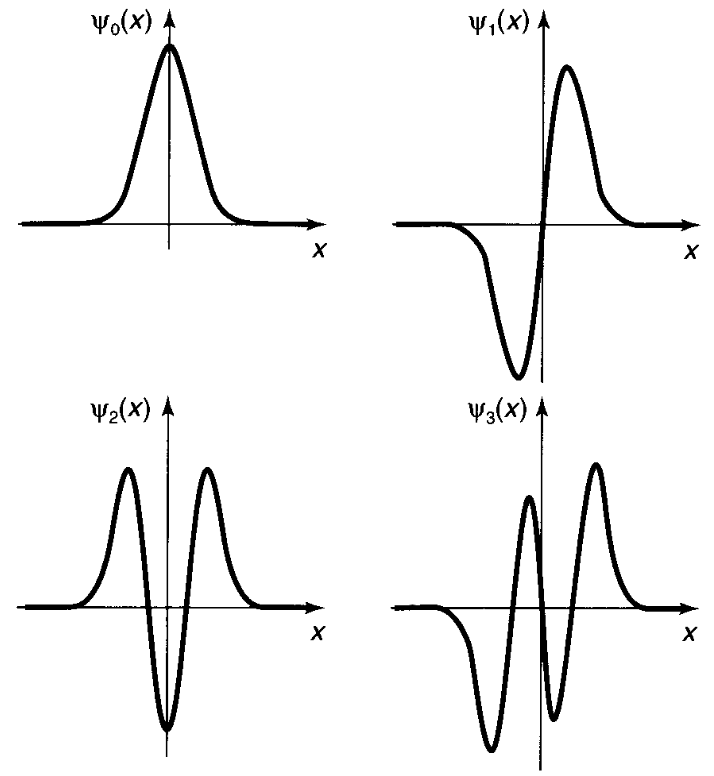
\includegraphics[width=0.6\textwidth]{armonico_func_onda}
    \caption{Primeras funciones de onda para el oscilador armónico}
    \label{fig:armonico_func_onda}
\end{figure}

Para el método algebraico reescribamos la ecuación de Schrödinger (ecuación \ref{eq:schrodinger_armonico}) de la siguiente forma
\begin{equation}
\frac{1}{2m} \left[\left(\frac{\hbar}{i} \frac{\mathrm{d}}{\mathrm{d}x}\right)^2 + (m \omega x)^2\right]\psi = E\psi
\label{eq:armonico_schrodinger_operador}
\end{equation}
donde la derivada es un operador sobre la función de onda $\psi$ \footnote{Para pasar a la notación de Dirac simplemente hay que recordar que $\psi = \langle x | \psi \rangle$}.
Por simpleza en la notación no consideramos el circunflejo caracteristico de los operadores, pero recorar que son operadores sobre autoestados o funciones de onda.

La ecuación \ref{eq:armonico_schrodinger_operador} nos está pidiendo a gritos factorizar, pero hay que tener cuidado porque son operadores.
Para eso definimos unos nuevos operadores
\begin{equation}
    a = \frac{1}{\sqrt{2m}} \left(\frac{\hbar}{i} \frac{\mathrm{d}}{\mathrm{d}x} - i m \omega x\right) \qquad 
    a^{\dagger} = \frac{1}{\sqrt{2m}} \left(\frac{\hbar}{i} \frac{\mathrm{d}}{\mathrm{d}x} + i m \omega x\right)
\end{equation}
es decir el operador y su autoadjuto.
Estos operadores no son hermíticos, pero si le aplicamos una función cualquiera al producto $a^{\dagger}a$ obtenemos
\[ (a^{\dagger}a) f(x) =  \frac{1}{2m} \left(\frac{\hbar}{i} \frac{\mathrm{d}}{\mathrm{d}x} + i m \omega x\right) \left(\frac{\hbar}{i} \frac{\mathrm{d}}{\mathrm{d}x} - i m \omega x\right) f(x)\]
\[ =  \frac{1}{2m} \left(\frac{\hbar}{i} \frac{\mathrm{d}}{\mathrm{d}x} + i m \omega x\right) \left(\frac{\hbar}{i} \frac{\mathrm{d} f}{\mathrm{d}x} - i m \omega x f\right) \]
\[ =  \frac{1}{2m} \left(- \hbar^2 \frac{\mathrm{d}^2 f}{\mathrm{d}x^2} - \hbar m \omega \frac{\mathrm{d} (x f)}{\mathrm{d}x} + \hbar m  \omega x \frac{\mathrm{d}f}{\mathrm{d}x} + (m \omega x)^2 f\right) \]
\[ = \frac{1}{2m} \left[ \left(\frac{\hbar}{i} \frac{d}{dx}\right)^2 + (m \omega x)^2 - \hbar m \omega\right] f(x) \]
donde usamos regla de la cadena para $\mathrm{d}(x f)/\mathrm{d}x$.
Si eliminamos la función de prueba nos queda
\begin{equation}
    a^{\dagger} a = \frac{1}{2m} \left[\left(\frac{\hbar}{i} \frac{\mathrm{d}}{\mathrm{d}x}\right)^2 + (m \omega x)^2\right] - \frac{\hbar \omega}{2}
\end{equation}
por lo que el hamiltoneano del oscilador queda
\begin{equation}
    (a^{\dagger}a + \frac{1}{2}\hbar \omega) \psi = E \psi
\end{equation}
Si en vez queremos usar el producto $a a^\dagger$ tenemos que la ecuación queda
\begin{equation}
    \left(a a^{\dagger} - \frac{\hbar \omega}{2} \right)\psi = E \psi
\end{equation}
El paso crucial consiste en demostrar que si $\psi$ verifica la ecuación de Schrödinger con energía $E$, entonces $a^{\dagger} \psi$ la verifica con $(E + \hbar \omega)$
\[ (a^{\dagger} a + \frac{\hbar\omega}{2} \psi) (a^{\dagger} \psi) = a^{\dagger} (a a^{\dagger} + \frac{\hbar\omega}{2}) \psi = a^{\dagger} \left[\left(a a^\dagger - \frac{1}{2}\hbar \omega \right)\psi - \hbar \omega \psi \right] = a^{\dagger} (E \psi + \hbar\omega \psi) = (E + \hbar \omega)(a^{\dagger}\psi) \]

Con esto podemos llamar al operador $a^{\dagger}$ como operador de creación o de subida, y al operador $a$ como operador de destrucción o de bajada.

Es notable que si aplicamos el operador de bajada de forma repetida podemos llegar a tener energía nula.
Para eso pedimos que exista una solución tal que
\begin{equation}
    a \psi_0 = \frac{1}{2m} \left[\frac{\hbar}{i} \frac{\mathrm{d}\psi_0}{\mathrm{d}x} - i m \omega x \psi_0 \right] = 0
\end{equation}
que se puede resolver por simple integración en
\begin{equation}
    \psi_0 = A_0 e^{-\frac{m \omega}{2\hbar} x^2}
\end{equation}
con autoenergía
\begin{equation}
    E_0 = \frac{\hbar\omega}{2}
\end{equation}

Definido la función de onda del fundamental las siguientes funciones de onda serán
\begin{equation}
    \psi_n(x) = \left(\frac{m \omega}{\pi \hbar}\right)^{1/4} \frac{(-i)^n}{\sqrt{n!(\hbar \omega)^n}} (a^\dagger)^n e^{-\frac{m \omega}{2\hbar} x^2}
\end{equation}
con energía
\begin{equation}
    E_n = \left(n + \frac{1}{2}\right) \hbar \omega
\end{equation}

Los operadores de subida y bajada también son
\begin{equation}
    a = \sqrt{\frac{m \omega}{2 \hbar}} x + i \sqrt{\frac{1}{m \omega \hbar}} \\ a^{\dagger} =  \sqrt{\frac{m \omega}{2 \hbar}} x - i \sqrt{\frac{1}{m \omega \hbar}}
\end{equation}

Y si definimos el operador número
\begin{equation}
    N = a^\dagger a
\end{equation}
con la siguiente propiedad
\begin{equation}
    N |n\rangle = n |n\rangle \qquad \langle x | n \rangle = \psi_n(x)
\end{equation}
por lo que el hamiltoneano queda
\begin{equation}
    H = \hbar \omega \left(N + \frac{1}{2}\right)
\end{equation}

Ahora veamos el conmutador de ellos, que nos permitirá usar el método para otros problemas
Antes hagamos el cambio de variable con $\xi$ a los operadores de subida y bajada
\begin{equation}
    a = \frac{1}{\sqrt{2}} \left[ \xi + \frac{\mathrm{d}}{\mathrm{d}\xi} \right] \qquad a^{\dagger} = \frac{1}{\sqrt{2}} \left[ \xi - \frac{\mathrm{d}}{\mathrm{d}\xi}\right]
\end{equation}
Con esto nos queda
\[ [a,a^\dagger] = a a^\dagger - a^\dagger a = \frac{1}{2} \left[ \left(\xi + \frac{\mathrm{d}}{\mathrm{d}\xi} \right) \left(\xi - \frac{\mathrm{d}}{\mathrm{d}\xi} \right) - \left(\xi - \frac{\mathrm{d}}{\mathrm{d}\xi}\right) \left( \xi + \frac{\mathrm{d}}{\mathrm{d}\xi} \right)\right] = \frac{\mathrm{d}}{\mathrm{d}\xi} (\xi) - \xi \frac{\mathrm{d}}{\mathrm{d}\xi}\]
si se lo aplicamos a una función de $\xi$ cualquiera obtenemos la función nuevamente, por lo que
\begin{equation}
    [a, a^{\dagger}] = 1
\end{equation}

Esto nos permite encontrar que
\[ a^\dagger a a^\dagger |n\rangle =  a^\dagger (a a^\dagger) |n \rangle = a^\dagger (a a^\dagger - a^\dagger a + a^\dagger a) |n \rangle = a^\dagger (1 + n) |n\rangle = (n + 1) a^\dagger |n\rangle\]
Que es lo que ya vimos con el operador de subida, pero deducido solamente con el conmutador.
Acá queda claro que los conmutadores nos permiten resolver el problema, solamente con el cambio de variable adecuado, sin pasar por la complicaciones de la función de onda, pero por completitud presentamos ambos métodos.

Los operadores $a$ y $a^\dagger$ no son hermíticos y ni siquiera son diagonales, ya que (mediante normalización)
\begin{equation}
    a^\dagger |n \rangle = \sqrt{n + 1} |n + 1\rangle \qquad a|n\rangle = \sqrt{n} |n - 1\rangle
\end{equation}

\section{Momento angular}

El momento angular en mecánica cuántica se define a partir de la definión clásica
\begin{equation}
    \hat{\boldsymbol{L}} = \hat{\boldsymbol{r}} \times \hat{\boldsymbol{p}} = \frac{\hbar}{i} \hat{\boldsymbol{r}} \times \hat{\nabla}
    \label{eq:momento_angular_def}
\end{equation}
Si definimos al producto vectorial con el simbolo de Levi Civita tenemos
\begin{equation}
    \hat{L}_i = \frac{\hbar}{i} \epsilon_{i j k}  \hat{r}_j \hat{p}_k
\end{equation}

Con la expresión anterior calculemos el conmutador entre componentes del momento angular
\[ [\hat{L}_i, \hat{L}_j] = [\epsilon_{i k l} \hat{r}_k \hat{p}_l, \epsilon_{j m n} \hat{r}_m \hat{p}_m] =  \epsilon_{i k l} \epsilon_{j m n} [\hat{r}_k \hat{p}_l, \hat{r}_m \hat{p}_n] = \epsilon_{i k l} \epsilon_{j m n} ([\hat{r}_k,\hat{r}_m \hat{p}_n] \hat{p}_l + \hat{r}_k [\hat{p}_l, \hat{r}_m \hat{p}_n]) \]
\[ = \epsilon_{i k l} \epsilon_{j m n} (\hat{r}_m [\hat{r}_k, \hat{p}_n]        \hat{p}_l + \hat{r}_k [\hat{p}_l, \hat{r}_m] \hat{p}_n) = \epsilon_{i k l} \epsilon_{j m n} (i \hbar \delta_{k n} \hat{r}_m \hat{p}_l + i \hbar \delta_{l m} \hat{r}_k \hat{p}_n) \] 
\[ = i \hbar \epsilon_{i k l} (\epsilon_{j m l} \hat{r}_m \hat{p}_l + \epsilon_{j l n}  \hat{r}_k \hat{p}_n) = i \hbar (\epsilon_{l i k} \epsilon_{l j m} \hat{r}_m \hat{p}_l + \epsilon_{l i k} \epsilon_{l j m} \hat{r}_k \hat{p}_n)\] 
Si usamos que 
\begin{equation}
    \epsilon_{ijk} \epsilon_{imn}=\delta_{j m} \delta_{kn} - \delta_{jn} \delta_{km}
\end{equation}
llegamos que
\begin{equation}
    [\hat{L}_i, \hat{L}_j] = i \hbar \epsilon_{i j k} L_k
\end{equation}

Esto último determina algo muy interesante propio de la cuántica: no se pueden medir con la misma precisión y en el mismo sitema las componentes del momento angular.

Es curioso, que si defino el operador $\hat{\boldsymbol{L}}^2$ como
\begin{equation}
    \hat{\boldsymbol{L}}^2 = \hat{L}^2_x+\hat{L}^2_y+\hat{L}^2_z = \hat{L}_i \hat{L}_i
\end{equation}
y calculo el conmutador con alguna componente
\[ [\hat{L}_i, \hat{\boldsymbol{L}}^2] = [\hat{L}_i, \hat{L}_j \hat{L}_j] = \hat{L}_j [\hat{L}_i, \hat{L}_j] + [\hat{L}_i, \hat{L}_j] \hat{L}_j = i \hbar (\epsilon_{i j k} \hat{L}_j \hat{L}_k + \epsilon_{i j k} \hat{L}_k \hat{L}_j)\]
que, si recordamos el simbolo de Levi Civita es antisimétrico y los operadores $\hat{L}_i$ no conmutan, resultando en 
\begin{equation}
    [\hat{L}_i, \hat{\boldsymbol{L}}^2] = 0
\end{equation}

Entonces para poder describir el momento angular vamos a necesitar una componente (que en general se elige $\hat{L}_z$) y el módulo, ya que conmutan y tienen una base de estados compatibles.

Ahora con la definición del momento angular (ecuación \ref{eq:momento_angular_def}) y la expresión del vector posición y el gradiente en esféricas tengo que
\begin{equation}
    \hat{\boldsymbol{L}} = \frac{\hbar}{i} \left[ \boldsymbol{\phi} \frac{\partial}{\partial \theta} - \boldsymbol{\theta} \frac{1}{\sen(\theta)} \frac{\partial}{\partial \phi} \right]
\end{equation}
del cual podemos deducir que la componente $\hat{L}_z$ es
\begin{equation}
    \hat{L}_z = \frac{\hbar}{i} \frac{\partial}{\partial \phi}
\end{equation}

Lo mismo podemos hacer para el operador $\hat{\boldsymbol{L}}^2$, usando la parte angular del laplaciano $\nabla^2$
\begin{equation}
\hat{\boldsymbol{L}}^2 = - \hbar^2  \left[ \frac{1}{\sen(\theta)} \frac{\partial}{\partial \theta} \left(\sen(\theta \frac{\partial}{\partial \theta} \right) + \frac{1}{\sen^2(\theta)} \frac{\partial^2}{\partial \phi^2} \right]
\end{equation}

Ahora construyamos dos operadores, de subida y bajada
\begin{equation}
    \hat{L}_{\pm} = \hat{L}_x \pm i \hat{L}_y
\end{equation}
que naturalmente conmuta con $\hat{\boldsymbol{L}}^2$
\begin{equation}
    [\hat{\boldsymbol{L}}^2, \hat{L}_\pm] = 0
\end{equation}
y el conmutador con $\hat{L}_z$ es
\[ [\hat{L}_z, \hat{L}_\pm ] = [\hat{L}_z, \hat{L}_x] \pm i [\hat{L}_z, \hat{L}_y] = i\hbar \hat{L}_y \pm i (-i\hbar \hat{L}_x) = \pm \hbar (\hat{L}_x \pm i \hat{L}_y)\]
es decir
\begin{equation}
    [\hat{L}_z, \hat{L}_\pm ] = \pm \hbar \hat{L}_\pm
\end{equation}

Para completar, podemos ver que la expresión en base de esféricas
\begin{equation}
    \langle \phi, \theta | \hat{L}_\pm | \psi \rangle = - i \hbar e^{\pm i \phi}\left(\pm i \frac{\partial}{\partial \theta} - \cot(\theta) \frac{\partial}{\partial \phi} \right) \langle \phi, \theta | \psi \rangle
    \label{eq:momento_operador_subibda_coordeanas}
\end{equation}

Si tenemos un estado $|\psi\rangle$ tal que
\begin{equation}
    \hat{\boldsymbol{L}}^2 |\psi\rangle = \lambda |\psi\rangle \qquad \hat{L}_z |\psi\rangle = \mu |\psi\rangle
\end{equation}
entonces veamos que produce el operador $\hat{L}_\pm$ a los autoestados del momento angular
\[\hat{\boldsymbol{L}}^2 (\hat{L}_\pm |\psi\rangle = \hat{L}_\pm (\hat{\boldsymbol{L}}^2 |\psi\rangle) = \lambda \hat{L}_\pm |\psi\rangle \]
y para $\hat{L}_z$
\[\hat{L}_z \hat{L}_\pm |\psi\rangle = (\hat{L}_\pm \hat{L}_z - [\hat{L}_z, \hat{L}_\pm]) |\psi\rangle = \hat{L}_\pm (\hat{L}_z \pm \hbar) |\psi\rangle = (\mu \pm \hbar) (\hat{L}_\pm |\psi\rangle) \]

Ahora pedimos que exista un estado superior e inferior tal que
\[ \hat{L}_+ |\psi^f\rangle = 0 \qquad \hat{L}_- |\psi^f\rangle = 0 \]
esos estados tienen los siguientes autovalores
\[ \hat{L}_z |\psi^f\rangle = \hbar l |\psi^f\rangle \qquad \hat{\boldsymbol{L}}^2 |\psi\rangle = \lambda |\psi^f\rangle \]

Para seguir escribimos el operador $\hat{\boldsymbol{L}}^2$ como suma de los otros
\begin{equation}
    \hat{\boldsymbol{L}}^2 = \hat{L}_\pm \hat{L}_\mp + \hat{L}^2_z \mp \hbar \hat{L}_z
\end{equation}

Si se lo aplicamos al estado $|\psi \rangle$ 
\[ \hat{\boldsymbol{L}}^2 |\psi\rangle = (\hat{L}_- \hat{L}_+ + \hat{L}_z + \hbar \hat{L}_z) |\psi\rangle = (0 + \hbar^2 l^2 + \hbar l)|\psi\rangle = \hbar^2 l(l + 1) |\psi\rangle \]

Si hacemos lo mismo para el estado inferior, pidiendo antes que $\hat{L}_z |\psi^b\rangle = \hbar \tilde{l} |\psi^b\rangle$
\[ \hat{\boldsymbol{L}}^2 |\psi^b\rangle = \hbar^2 \tilde{l} (\tilde{l} - 1) |\psi^b\rangle\]

Los autovalores de $\hat{\boldsymbol{L}}^2$ son independientes de los valores de subida y bajada, como ya vimos, por lo que la única solución posible para $l$ es que
\[ \tilde{l} = - l \]
y evidentemente los operadores $\hat{L}_z$ y $\hat{\boldsymbol{L}}^2$ tienen la siguiente propiedad
\begin{equation}
    \hat{L}_z |\psi\rangle = \hbar m |\psi\rangle \qquad \hat{\boldsymbol{L}}^2 |\psi\rangle = \hbar^2 l( l + 1) |\psi\rangle
\end{equation}
con
\begin{equation}
    m \in [-l, l]
\end{equation}
con $N$ valores diferentes de $m$ entre $[-l, l]$, lo que conlleva a decir que $l = -l + N$, con $N = l/2$
\begin{equation}
    l \in \{0, 1/2, 1, 3/2, 2, \dots\} \qquad m \in \{ -l, -l + 1, \dots, l - 1, l\}
\end{equation}

Y los los estados los vamos a escribir como
\begin{equation}
    |\psi\rangle = |l, m\rangle
\end{equation}
si tienen el momento angular definido.

Para encontrar las autofunciones podemos usar la expresión de los operadores $\hat{\boldsymbol{L}}^2$ y $\hat{L}_z$ como vamos a hacer en el próximo apartado, o podemos usar los operadores de subida y bajada, que para el estado $|l, l \rangle$ el de subida tiene una expresión simple, y construyendolo de forma recursiva.
La ventaja de este método es que no hay que resolver ecuaciones diferenciales complicadas.

\subsection{Rotaciones infinitesimales y sus generadores}

Veamos como relacionamos una rotación rígida, que parametrizamos con un vector $\textbf{a}$, y el momento angular.
Para eso tenemos una función escalar $\phi(\textbf{r})$ con la que construimos una nueva función $\Phi$ tal que
\[ \Phi(\boldsymbol{r} + \boldsymbol{a}) = \phi(\boldsymbol{r}) \]
Si el vector $\textbf{a}$ es una rotación de un ángulo infinitesimal $\delta \varphi$ tengo que
\[ \textbf{a} = \delta\boldsymbol{\varphi} \times \boldsymbol{r}\]
y la tranformación infinitesimal de la función escalar es
\[ \delta \phi = \Phi(\textbf{r}) - \phi(\textbf{r}) = \delta \textbf{a} \dot \nabla \phi(\textbf{r}) = - (\delta \boldsymbol{\varphi} \times \textbf{r}) \dot \nabla \phi = - \delta \boldsymbol{\varphi} \dot (\textbf{r}\time\nabla) \phi(\textbf{r})\]
donde el operador que queda expresado corresponde a
\begin{equation}
    \delta \phi = -\frac{i}{\hbar} \delta \boldsymbol{\varphi} \dot \hat{\textbf{L}} \phi(\textbf{r})
\end{equation}

Esto último determina que el generador de las rotaciones infinitesimales (y por lo tanto de rotaciones general) es el operador momento angular. 
Esto se puede generalizar para cualquier tipo de momento, y además puede ser usado como definición del momento angular y deducir las relaciones de conmutación.

\subsection{Autofunciones}
Ahora resolvamos la ecuación 
\begin{equation}
    \hat{\boldsymbol{L}}^2 |l,m\rangle = \hbar^2 l(l + 1) |l, m\rangle
\end{equation}
multiplicando por el bra $\langle \phi, \theta|$ que corresponde escribir la ecuación diferencial es esféricas
\begin{equation}
    \frac{1}{\sen(\theta)} \frac{\partial}{\partial \theta} \left(\sen(\theta) \frac{\partial}{\partial \theta} f(\theta, \phi) \right) + \frac{1}{\sen^2(\theta)} \frac{\partial^2}{\partial \phi^2} f(\theta, \phi) = - l (l + 1) f(\theta, \phi)
\end{equation}
si multiplico $\sen^2(\theta)$ a ambos lados obtengo
\begin{equation}
    \sen(\theta) \frac{\partial}{\partial \theta} \left(\sen(\theta) \frac{\partial}{\partial \theta} f(\theta, \phi) \right) +  \frac{\partial^2}{\partial \phi^2} f(\theta, \phi) =  -  l (l + 1) \sen^2(\theta) f(\theta, \phi)
    \label{eq:momento_angular_laplace}
\end{equation}
Esta ecuación corresponde a la parte angular de la ecuación de Laplace
\begin{equation}
    \nabla^2 f = \frac{1}{r^2} \frac{\partial}{\partial r}\left( r^2 \frac{\partial f}{\partial r} \right) + \frac{1}{r^2 \sen(\phi)} \frac{\partial}{\partial \phi} \left( \sen(\phi) \frac{\partial f}{ \partial \phi} \right) + \frac{1}{r^2 \sin^2 \phi} \frac{\partial^2 u}{\partial \theta^2} = 0
\end{equation}
con la constante de separación igual a $l(l + 1)$.
Para resolver la ecuación \ref{eq:momento_angular_laplace} proponemos
\begin{equation}
    f(\theta, \phi) = Y_{l m}(\theta, \phi) = \Theta(\theta) \Phi(\phi)
\end{equation}
Con esta propuesta y dividiendo por $\Theta \Phi$ (como se produce en la mayoría de las ecuaciones separables) llegamos  a 
\begin{equation}
    \left\{ \frac{1}{\Theta} \sen(\theta) \frac{\mathrm{d}}{\mathrm{d}\theta} \left(\sen(\theta) \frac{\mathrm{d}\Theta}{\mathrm{d}\theta}\right) + l (l + 1) \sen^2(\theta) \right\} + \frac{1}{\Phi} \frac{\mathrm{d}^2 \Phi}{\mathrm{d}\phi^2} = 0
\end{equation}
que podemos resolver nuevamente por separación con la constante $m^2$
\begin{equation}
    \begin{gathered}
    \sen(\theta) \frac{\mathrm{d}}{\mathrm{d}\theta} \left(\sen(\theta) \frac{\mathrm{d}\Theta}{\mathrm{d}\theta}\right) + [l (l + 1) \sen^2(\theta) - m^2] \Theta = 0 \\ 
    \frac{\mathrm{d}^2 \Phi}{\mathrm{d}\phi^2} = - m^2 \Phi
\end{gathered}
\end{equation}

La parte polar es fácil de resolver
\begin{equation}
    \Phi = e^{i m \phi}
\end{equation}
con la constante en la otra función.
Elegimos solamente la solución positiva porque permitimos que $m$ tenga valores negativos. 
Además si pedimos continuidad 
\begin{equation}
    \Phi(\phi + 2\pi) = \Phi(\phi)
\end{equation}
llegamos a que 
\begin{equation}
    m \in \mathbb{Z}
\end{equation}
Mientras que la parte azimutal tiene como solución 
\begin{equation}
    \Theta(\theta) = A P^{m}_l(\cos(\theta))
\end{equation}
con $P^{m}_l$ los polinomios de Legendre asociados, definidos como
\begin{equation}
    P^{m}_l(x) = (1 - x^2)^{|m|/2} \left(\frac{\mathrm{d}}{\mathrm{d}x}\right)^{|m|} P_l(x)
    \end{equation}
y los polinomios de Legendre los podemos definir con la fórmula de Rodrigues
\begin{equation}
    P_l(x) = \frac{1}{2^l l!} \left(\frac{\mathrm{d}}{\mathrm{d}x}\right)^{l} (x^2 - 1)^l
\end{equation}
Finalmente podemos deducir las reglas para $l$ y $m$ usando que la $n$-esima derivada  de cualquier polinomio de grado $n'$ es nula si $n > n'$
\begin{equation}
    l \in \mathbb{N}^0 \qquad m \in [-l, l], m \in \mathbb{Z}
\end{equation}

Esto último es muy interesante, ya que ya encontramos que $m$ y $l$ pueden ser semi enteros, pero para el momento angular orbital no puede ser el caso. 
Esto puede significar la existencia de una magnitud física asociada al momento angular, que experimentalmente se encontró y se denominó \emph{spin}, por ser un momento angular intrínseco.
Recién en la teoría relativista se le dió significado al momento angular intríseco

Finalmente las funciones normalizadas serán
\begin{equation}
    Y^{m}_l = \epsilon \sqrt{\frac{2l + 1}{4\pi} \frac{(l - |m|)!}{(l + |m|)!}} e^{i m \phi} P^{m}_l(\cos(\theta))
\end{equation}
con $\epsilon = (-1)^m$ si $m \geq 0$ o $\epsilon = 1$ si $m \leq 0$.

\section{Fuerzas centrales}
Es interesante observar el problema de fuerzas centrales, o que con el mismo proceso algebraico es equivalente al problema de dos cuerpos, que tiene el siguiente hamiltoneano
\begin{equation}
    \hat{H} = \frac{\hat{\boldsymbol{p}}^2}{2m} + V(\hat{\boldsymbol{r}})
\end{equation}
El operador momento lineal en este caso representa el laplaciano, que vamos a escribirlo en esféricas.
\begin{equation}
    \langle \boldsymbol{r}|\hat{H}|\psi\rangle = \frac{-\hbar^2}{2m} \nabla^2 \psi(\boldsymbol{r}) + V(\textbf{r}) \psi(\boldsymbol(r)) = E \psi(\textbf{r}) 
\end{equation}

Como el potencial sólo depende de la posición, entonces podemos separar en parte radial y parte angular, pero la parte angular ya la resolvimos para el momento angular.
De esta forma todo potencial central tiene la misma parte angular, los armónicos esféricos, y diferente parte radial depediendo de la forma del potencial.

Usando la misma constante de separación para la parte angular (a saber $l (l + 1)$) tenemos que la parte radial $R(r)$ de la función de onda verifica
\begin{equation}
    \frac{\mathrm{d}}{\mathrm{d}r} \left(r^2 \frac{\mathrm{d} R}{\mathrm{d}r} \right) - \frac{2 m r^2}{\hbar^2} (V(r) - E - l(l + 1)) R = 0
\end{equation}

Para resolver esta ecuación proponemos el cambio de variable $u = R/r$
\begin{equation}
    -\frac{\hbar^2}{2m} \frac{\mathrm{d}^2 u}{\mathrm{d}r^2} + \left[ V(r) + \frac{\hbar^2}{2m} \frac{l (l + 1)}{r^2} \right] u = E u
    \label{eq:central_ec_radial}
\end{equation}
que se denomina ecuación radial.


\subsection{Átomo de hidrógeno}
El átomo de hidrógeno es un caso particular de fuerzas centrales, en el cual podemos considerar que la masa del nucleo está quieta (o no, y ahí debemos pensar en una masa reducida $\mu$) y el electrón orbitando con el siguiente potencial central
\begin{equation}
    V(r) = -\frac{e^2}{r}
\end{equation}
donde usamos unidades gaussianas ($\epsilon_0 = \frac{1}{4\pi}$).
La ecuación radial (ecuación \ref{eq:central_ec_radial}) queda
\begin{equation}
    -\frac{\hbar^2}{2m} \frac{\mathrm{d}^2 u}{\mathrm{d}r^2} + \left[ - \frac{e^2}{r} + \frac{\hbar^2}{2m} \frac{l (l + 1)}{r^2} \right] u = E u
\end{equation}
Si ahora rescribimos las constantes con $\kappa = \frac{\sqrt{-2mE}}{\hbar}$ tenemos
\[\frac{1}{\kappa^2} \frac{\mathrm{d}^2 u}{\mathrm{d} r^2} = \left[1 - \frac{m e^2}{2 \hbar^2 \kappa} \frac{1}{\kappa r} + \frac{l (l + 1)}{(\kappa r)^2} \right] u\]
Con el cambio de variables $\rho = \kappa r$ y $\rho_0 = \frac{m e^2}{2 \hbar^2 \kappa}$ tenemos
\begin{equation}
    \frac{\mathrm{d}^2 u}{\mathrm{d}\rho} = \left[1 - \frac{\rho_0}{\rho} + \frac{l(l + 1)}{\rho^2}\right] u
\end{equation}

Para resolver la ecuación anterior veamos el comportamiento para $\rho \to 0$ y para $\rho \to \infty$
\begin{equation}
    \begin{gathered}
        \rho \to 0 \implies \frac{\mathrm{d}^2 u}{\mathrm{d} \rho^2} \approx \frac{l(l + 1)}{\rho^2} u\\
        \rho \to \infty \implies \frac{\mathrm{d}^2 u}{\mathrm{d} \rho^2} = u
    \end{gathered}
\end{equation}

Las soluciones posibles a estas ecuaciones son
\begin{equation}
    \begin{gathered}
        \rho \to \infty  \implies u(\rho) = A e^{-\rho} + B e^{\rho} \\
        \rho \to 0 \implies u(\rho) = C \rho^{l + 1} + D \rho^{-l}
    \end{gathered}
\end{equation}
y si eliminamos las divergencias, a la vez que si observamos que tener el producto de ambas soluciones asintóticas también da el mismo comportamiento asintótico, sólo nos queda encontrar la función que empalme ambas soluciones
\begin{equation}
    u(\rho) = \rho^{l + 1} e^{-\rho} v(\rho)
\end{equation}

De esta forma la ecuación para $v(\rho)$, que corresponde a la ecuación radial con el reemplazo de la función de prueba, será
\begin{equation}
    \rho \frac{\mathrm{d}^2 v}{\mathrm{d}\rho^2} + 2(l + 1 - \rho) \frac{\mathrm{d} v}{\mathrm{d}\rho} + [\rho_0 - 2(l + 1)] v = 0
\end{equation}
Si en esta ecuación pruebo una serie de potencia
\begin{equation}
    v(\rho) = \sum_{j = 0}^\infty a_j \rho^j
\end{equation}
y obtenemos una relación de recurrencia calculando las derivadas pertinentes en la ecuación diferencial
\begin{equation}
    a_{j + 1} = \left[ \frac{ 2(j + l + 1) - \rho_0}{(j + 1) (j + 2l + 2)}\right] a_j
\end{equation}
Nuevamente si observamos el comportamiento asintótico de los coeficientes encontramos que debe terminar, es decir que exista un valor para el cual $a_{j + 1} = 0$, que es evidentemente
\begin{equation}
    2 (j_{max} + l + 1) - \rho_0 = 0
\end{equation}
y si definimos 
\begin{equation}
    n = j_{\max} + l + 1
\end{equation}
como un número entero, por lo tanto los valores de $l$ serán
\begin{equation}
    l \in \{0, 1, 2, \dots, n - 1\}
\end{equation}
y además podemos encontrar la energía, sabiendo que 
\[ \rho_0 = \frac{m e^2}{2 \hbar \sqrt{-2 m E}} = 2n\]
por lo que finalmente (recordando que $\kappa = \frac{\sqrt{-2 m E}}{\hbar}$
\begin{equation}
    E = - \frac{m e^4}{2 \hbar^2} \frac{1}{n^2} = \frac{E_1}{n^2}
\end{equation}
que corresponde a la energía encontrada por Bohr años antes de resuelta la ecuación de Schröndinger.

La función $v(\rho)$ corresponde a 
\begin{equation}
    v(\rho) = L^{2l + 1}_{n - l -1}(2\rho)
\end{equation}
siendo el simbolo ese
\begin{equation}
    L^{p}_{q - p}(x) = (-1)^p \left(\frac{\mathrm{d}}{\mathrm{d}x}\right)^p L_q(x)
\end{equation}
un polinomios de Laguerre asociado, y
\begin{equation}
    L_q(x) = e^x \left(\frac{\mathrm{d} (e^-x x^q)}{\mathrm{d}x}\right)^q
\end{equation}
los polinomios de Laguerre.

Para completar presentamos las autofunciones normalizadas

\begin{equation}
    \psi_{nlm}(r,\phi,\theta) = \sqrt{\left(\frac{2}{n a}\right)^3 \frac{(n - l - 1)!}{2n[(n + l)!]^3}} e^{-r/(na)} \left(\frac{2r}{na}\right)^l L^{2l + 1}_{n - l - 1}\left(\frac{2r}{na}\right) Y^{m}_{l}(\theta, \phi)
\end{equation}

con $a$ el radio de Bohr
\begin{equation}
    a = \frac{\hbar^2}{m e^2} = 0,529 \times 10^{-10}\;\text{m}
\end{equation}
que corresponde al radio de la primera orbita.
Este radio también se puede encontrar invocando al principio de incertidumbre.

%\subsection{Suma de momento angular}

%Dos estados de momento angular definido podemos sumarlos de forma desacoplada, es decir
%\begin{equation}
%  |j_1,j_2,m_1,m_2\rangle = |j_1,m_1\rangle \otimes |j_2,m_2\rangle
%\end{equation}

%El cambio de base, a la descripción acoplada, corresponde a
%\begin{equation}
%  |j,m\rangle = \sum_i |j_1,j_2,m_1,m_2\rangle \langle j_1,j_2,m_1,m_2|j,m\rangle
%\end{equation}

\section{Spin}

En mecánica clásica existen dos tipos de momento angular, el momento angular orbital, $\boldsymbol{L}$ respecto algún punto y el momento angular intrínseco, $\boldsymbol{S}$ llamado spin en inglés, que representa el momento angular orbital de las partes del sistema respecto al centro de masa.
Siguiendo el programa de la mecánica cuántica, definimos el momento angular orbital, $\hat{\boldsymbol{L}}$, con todas sus sutilezas, y observamos como la resolución algebraica permitía autoestados con valores $l$ semienteros, que podemos con la resolución analítica encontramos que no tienen representación en el espacio de coordenadas.
Esto nos está diciendo la existencia de un momento angular que si puede tomar $l$ como semientero, pero necesita un fundamento experimental.

En varias experiecias, en particular las de Stern y Gerlach (que se observa en la figura \ref{fig:stern_gerlach}) que demostró la existencia de un momento angular intrínseco al observar un momento dipolar magnético intrínseco.

\begin{figure}[H]
    \centering
%\includegraphics{}
    \caption{Caption}
    \label{fig:stern_gerlach}
\end{figure}

Asumido que existe este operador, que llamamos \emph{spin}, podemos usar toda la teoría algebraica del momento angular para explicarlo, empezando con las reglas de conmutación
\begin{equation}
        [\hat{S}_i, \hat{S}_j] = i \hbar \epsilon_{ijk} \hat{S}_k \qquad [\hat{S}_i, \hat{S}^2] = 0
\end{equation}
con lo que podemos deducir que los autoestados de los operadores  son
\begin{equation}
\hat{S}_z |s,m\rangle = \hbar m |s,m\rangle \qquad \hat{S}^2 |s, m\rangle = \hbar^2 s(s + 1) |s,m\rangle
\end{equation}
También agregamos los operadores de subida y bajada
\begin{equation}
 \hat{S}_\pm = \hat{S}_x \pm i \hat{S}_y
\end{equation}
con la siguiente propiedad
\begin{equation}
\hat{S}_\pm |s, m\rangle = \sqrt{s(s+1) - m( m \pm 1)} |s, m \pm 1 \rangle 
\end{equation}

Para el spin de $1/2$, tenemos dos estados
\begin{equation}
    s = \frac{1}{2} \implies |s,m\rangle \in \left\{\left|\frac{1}{2},\frac{1}{2}\right.\rangle, \left|\frac{1}{2},-\frac{1}{2}\right.\rangle\right\}
\end{equation}
Estos estados los podemos expresar en forma matricial como
\begin{equation}
|1/2,1/2\rangle = \begin{pmatrix} 1 \\ 0 \end{pmatrix} \qquad |1/2,-1/2\rangle = \begin{pmatrix} 0 \\ 1 \end{pmatrix}
\end{equation}
Un estado general se puede expresar por lo tanto
\begin{equation}
    \xi = \begin{pmatrix} a \\ b \end{pmatrix}
\end{equation}
Estos elementos de matrix se denomina espinores, porque al rotarlos $2\pi$ cambian de signo (usando la rotación inducida por el operador $\hat{\boldsymbol{S}}$).

Si escribimos los operadores $\hat{S}_i$ y $\hat{S}^2$ con esta notación obtenemos
\begin{equation}
    \begin{gathered}
        \hat{S}_z = \frac{\hbar}{2} \begin{pmatrix} 1 & 0 \\ 0 & -1 \end{pmatrix} \qquad
        \hat{S}_x = \frac{\hbar}{2}\begin{pmatrix} 0 & 1 \\ 1 & 0 \end{pmatrix}\\ 
    \hat{S}_y = i \begin{pmatrix} 0 & -1 \\ 1 & 0 \end{pmatrix} \qquad
    \hat{S}^2 = \frac{3}{2}\hbar \begin{pmatrix} 1 & 0 \\ 0 & 1 \end{pmatrix}
\end{gathered}
\end{equation}
Las matrices de $\hat{S}_x$ y $\hat{S}_y$, que las encontramos usando las expresiones de $\hat{S}_\pm$, son diagonales en los siguientes estados
\begin{equation}
    \begin{gathered}
    \hat{S}_x \text{ es  diagonal en } \left\{\frac{|+ \rangle + i |-\rangle}{\sqrt{2}}, \frac{|+\rangle - i |-\rangle}{\sqrt{2}}\right\} \\
    \hat{S}_y \text{ es  diagonal en } \left\{\frac{|+\rangle + |-\rangle}{\sqrt{2}}, \frac{|+\rangle - |-\rangle}{\sqrt{2}}\right\}
\end{gathered}
\end{equation}

Estas matrices son conocidas como de Pauli, y las matrices $\hat{S}_i$ y $\hat{S}^2$ son hermíticas (y observables), pero no así las $\hat{S}_\pm$
Lo mismo podemos hacer para spin de más dimensiones, lo único es necesario recordar la expresión de los operadores $\hat{S}_\pm$.
Acá se vuelve a mostrar la utilidad de este método con operadores.

\section{Estadísticas cuánticas}
  Los bosones (spin entero) exigen función de onda simétrica 
\begin{equation}
  P |\psi\rangle = |\psi\rangle
\end{equation}
mientras los fermiones (spin semientero) exigen
\begin{equation}
 P |\psi\rangle = - |\psi\rangle
\end{equation}
es decir función de onda antisimétrica
Dadas $n$ partículas con estados $|\psi_i(\alpha_i)\rangle$ (donde $\alpha_i$ es un parámetro del estado, como la posición), para construir el estado más general de fermiones tenemos el determinante de Slatter
\begin{equation}
  |\psi\rangle = \frac{1}{\sqrt{n}} \begin{vmatrix} |\psi_1(\alpha_1)\rangle & |\psi_2(\alpha_1)\rangle & \cdots & |\psi_n(\alpha_1)\rangle \\  |\psi_1(\alpha_2)\rangle & |\psi_2(\alpha_2)\rangle & \cdots & |\psi_n(\alpha_2)\rangle \\ \vdots & \vdots & \ddots & \vdots \\  |\psi_1(\alpha_n)\rangle & |\psi_2(\alpha_n)\rangle & \cdots & |\psi_n(\alpha_n)\rangle \end{vmatrix}
\end{equation}
y para bosones usamos el permanente de la matriz, como si fuese un determinante pero sin alternar los signos
\begin{equation}
   |\psi\rangle = \frac{1}{\sqrt{n}}\; \text{perm}\begin{pmatrix} |\psi_1(\alpha_1)\rangle & |\psi_2(\alpha_1)\rangle & \cdots & |\psi_n(\alpha_1)\rangle \\  |\psi_1(\alpha_2)\rangle & |\psi_2(\alpha_2)\rangle & \cdots & |\psi_n(\alpha_2)\rangle \\ \vdots & \vdots & \ddots & \vdots \\  |\psi_1(\alpha_n)\rangle & |\psi_2(\alpha_n)\rangle & \cdots & |\psi_n(\alpha_n)\rangle \end{pmatrix}
\end{equation}





\end{document}

